\documentclass[UKenglish]{ifimaster}
\usepackage[latin1]{inputenc}
\usepackage[T1]{fontenc,url}
\urlstyle{sf}
\usepackage{babel,textcomp,uiosloforside,varioref,graphicx}
\usepackage{color}
\usepackage[usenames,dvipsnames]{xcolor}

\newcommand{\todo}[1]{\textcolor{blue}{#1}}
\newcommand{\note}[1]{\textcolor{PineGreen}{\textbf{#1}}}
\newcommand{\question}[1]{\textcolor{red}{\textbf{#1}}}

\title{CloudML}
\subtitle{A DSL for model-based realization of applications in the cloud}
\author{Eirik Brandtz�g}
\date{Spring 2012}

\begin{document}
\uiosloforside[kind={Master thesis}]{}

\frontmatter{}
\maketitle{}
\textcolor{red}{\textbf{Built: \today}}

\chapter*{Abstract}

\tableofcontents{}
\listoffigures{}
\listoftables{}

\chapter*{Preface}

\mainmatter{}
\part{Introduction}

\section{Introduction (10)}

Short about my problem, why it's important and whats to be found in the thesis 

\begin{itemize}
  \item Summarize the \textbf{problem} \\
      Challenges from CloudMDE
    \begin{itemize}
      \item Information dependency at runtime
      \item Technical competence/level expectations
      \item Reproducibility
      \item Robustness
      \item Complexity
      \item Shareable
    \end{itemize}
  \item Short description of terms used
    \begin{itemize}
      \item Cloud (computing)
      \item Model-driven engineering
      \item Provider (cloud provider)
    \end{itemize}
  \item Why is it an important problem \\
      Ranting\ldots
    \begin{itemize}
      \item Cloud domain is state of the art
      \item model driven approach with benefits (no special tooling)
      \item Easier for businesses (especially SMBs) to reach out to Cloud
      \item Easier for larger more time-constraint businesses to try out the cloud
      \item Opening the eyes of big providers for a larger cross-cloud language
    \end{itemize}
  \item Shortly mention CloudML \\
      Summary from chap 3 in CloudMDE
  \item Shortly mention cloudml-engine \\
      Copy/paste implementation paragraph from CloudMDE
  \item Summarize chapters of thesis
\end{itemize}

\mychapter{background}{Background: Cloud computing and Model-Driven Engineering}
\begin{table}
  \begin{tabular}{ | l | l | l | }
    \hline
    \textbf{Provider} & \textbf{Service} & \textbf{Service layer} \\ \hline
    AWS & \emph{Elasic Compute Cloud}~(EC2) & IaaS \\ \hline
    AWS & Elastic Beanstalk & PaaS \\ \hline
    Google & \emph{Google App Engine}~(GAE) & PaaS \\ \hline
    Microsift & Azzure & PaaS and IaaS \\ \hline
    Heroku & Different services & PaaS \\ \hline
    Nodejitsu & Node.js & PaaS \\ \hline
    Rackspace & CloudServers & IaaS \\ \hline
  \end{tabular}
  \caption{Providers available services}
  \label{table:providerservices}
\end{table}


\begin{figure}
  \begin{center}
    \begin{tikzpicture}[scale=0.7, transform shape]
      \node (CloudServices) [class] { \textbf{Cloud Services} };
      \node (Instances) [class, below=of CloudServices] { \textbf{Instances} };

      \draw (CloudServices) -- (Instances);
    \end{tikzpicture}
  \end{center}
  \caption{Cloud layers}
  \label{fig:cloudlayers}
\end{figure}



In this chapter the essential background topics for this thesis is introduced,
that is cloud computing and Model-Driven architecture.

\section{Cloud computing}

Cloud computing is gaining popularity and more companies are starting 
to explore the possibilities as well as the limitation to the cloud.
The definitins under are mainly based on definitions by 
the \emph{National Institute of Standards and Technology}~(NIST) which is one of 
the leaders in cloud computing standardization.
The main providers of cloud computing at writing moment 
are Google, Amazon with \emph{Amazon Web Service}~(AWS)~\cite{aws} and Microsoft \todo{source?}.
A non-exhaustive list of common providers are visualized in \citetable{providerservices}.

\subsection{Characteristics}

Many characteristics of cloud computing is based on the ability to scale, both upwards and inwards.
Some of the most essential characteristics of cloud computing~\cite{nist:mell11} are:

\paragraph{On-demand self-service.} 

Consumers can do provisioning without any human interaction.
On-demand means dynamic scalability and elasticity of resource allocation,
self-service means that users does not need to manually do these allocations themselves.
Consider an online election system, for most of the year it will most likely have very
low usage demands, but before and under election days it will have to serve
a much larger amount of requests. With on-demand self-service the online election system
could automatically be given more resources such as memory, computation power or even
increase the number for instances to handle peak loads.
The previous example has planned (or known) peak intervals, so even though automatic handling
is appealing it could be solved by good planning. 
But sometimes predicting load peaks can be difficult, such as when a product suddenly
gets more popular.

\paragraph{Broad network access.}

Capabilities available over standard network mechanisms.
Supporting familiar protocols such as HTTP/HTTPS and SSH.
This means that users can utilize tools and software they are most likely already possesses
or will have little difficulty gaining, such as web browsers.
Most cloud providers also provide web based consoles/interfaces that users can use
to create, delete and manage their resources.

\paragraph{Resource pooling.}

Physical and virtual resources are pooled so they can be 
dynamically assigned and reassigned according to consumer demand.
This means users do not need to be troubled with scalability as this is handled automatically.
This is a provider side characteristic which directly influence \emph{on-demand self-service}.
There is also a sense of location independence, which means users do not have specific geographical
information about where resources are hosted from, only on higher levels of abstraction (country, state).

\paragraph{Rapid elasticity.}

Automatic capability scaling.
Already allocated resources can expand to meet new demands.
Towards the characteristic of \emph{on-demand self-service} this means that allocation
can happen instantly, which means on unexpected peak loads the pressure will be
instantly handled by scaling upwards.
It is important to underline that such features can be cost heavy if not limited,
because costs reflect resource allocation.
\paragraph{Measured service.}

Monitoring and control of resource usages.
Can be used for statistics for users, for instance to do analytical research on product popularity
or determine user groups based on geographical data or browser usage.
The providers themselves use this information to handle \emph{on-demand services},
if they notice that an instance has a peak in load or has a noticeable increase 
in requests they can automatically allocate more resources or capabilities 
to leave pressure.
\emph{Measuring} can also help providers with billing, if they for instance
charge by resource load and not only amount of resources allocated.

\subsection{Service models}

\emph{Service models} are definitions of different layers in cloud computing.
The layers represent the amount of abstraction developers get from each \emph{service model}.
Higher layers have more abstraction, but can be more limited, while lower levels 
have less abstraction and are more customizable.
Limitations could be in many different forms, such as bound to a specific operating system,
programming language or framework.
There are three main architectural service models in cloud computing\cite{nist:mell11}
as seen as vertical integration levels in \citefig{cloudlayers},
namely \emph{Infrastructure-as-a-Service}~(IaaS), \emph{Platform-as-a-Service}~(PaaS)
and \emph{Software-as-a-Service}~(SaaS).
IaaS is on the lowest closest to physical hardware and SaaS on the highest
level as runnable applications.

  \paragraph{IaaS.}

This layer is similar to more standard solutions such as \emph{Virtual Private Servers}~(VPS),
and is therefore the \emph{service model} closest to standard hosting solutions.
Stanoevska-Slabeva~\cite{introduction:wozniak10} emphasizes that
\emph{''infrastructure had been available as a service for quite some time``} and this 
\emph{''has been referred to as utility computing, such as Sun Grid Compute Utility``}.
Which means IaaS can also be compared to grid computing, 
a well known term in the academic world.
The NIST Definition of Cloud Computing~\cite{nist:mell11} define IaaS as
\epigraph{The capability provided to the consumer is to provision 
  processing, storage, networks, and other fundamental computing resources where the 
  consumer is able to deploy and run arbitrary software, which can include operating 
  systems and applications.
}{\todo{NIST, 2011}}
This underline the liberty this \emph{service model} provide users, but this also means
that developers need to handle software and tools them selves, from operating system and
up to their application. In some cases this is wanted, for instance when deploying 
native libraries and tools that applications rely on such as tools to convert and edit
images or video files. But in other cases this is not necessary and choosing this \emph{service model}
can be manpower in-effective for companies as developers must focus on meta tasks.
NIST continue to state that 
\epigraph{The consumer does not manage or control the underlying cloud 
  infrastructure but has control over operating systems, storage, deployed applications, and 
  possibly limited control of select networking components (\eg, host firewalls).
}{\todo{NIST, 2011}}
This means users have control over which operating system they want, in some cases users
can only pick from a set of pre-configured operating systems.
It is common for providers to include both Linux and Windows in their selections.
Some providers such as Amazon let users upload their own disk images.
A similarity to VPS is that operating systems are not manually installed,
when selecting an operating system this is copied directly into the instance pre-installed
and will therefore be instantly ready for usage.
Examples of providers of IaaS are AWS \emph{Elastic Compute Cloud}~(EC2) and Rackspace CloudServers.

\paragraph{PaaS.}

Cloud computing is built to guide and assist developers through abstractions, and the next
layer in the \emph{service model} is designed to aid developers by detaching them
from configuration of operating system and frameworks.
NIST state that developers will can \emph{``applications created using programming languages, 
libraries, services, and tools supported by the provider''}~\cite{nist:mell11}.
This means that developers are limited to these capabilities the provider support,
such as programming languages (Java, C\#), environments (JVM, .NET, Node.js), 
storage systems (flat files, NoSQL databases, RDBMS).
For example the first versions of \emph{Google App Engine}~(GAE) did only support
an internal key-value based database called BigTable, this is still their main database.
This database is transparently interfaced using their API, but also support technologies such as JPA and JDO,
this means users are bound to Java and these frameworks, and even limitations to the frameworks
as they have specific handlers for RDBMS.

PaaS providers support deployments through online APIs, in many cases by providing 
specific tools such as command line interfaces or plugins to IDEs like Eclipse.
It is common for the API to have client built on technologies related to the technology supported by the PaaS,
for instance Heroku has a Ruby-based client and Nodejitsu has an executable Node.js-module as client.

Examples of PaaS providers are Google with \emph{Google App Engine}~(GAE) and
the company Heroku with their service with the same name.
Amazon also entered the PaaS market with their service named Elastic Beanstalk,
which is an abstraction over EC2 as IaaS underneath.
Multiple PaaS providers utilize EC2 as underlying infrastructure, examples of such
providers are Heroku Nodester and Nodejitsu, this is a tendency with increasing popularity.

\paragraph{SaaS.}

The highest layer of the \emph{service models} farthest away from physical hardware
and with highest level of abstraction.
NIST describe SaaS as
\epigraph{The capability provided to the consumer is to use the provider's 
  applications running on a cloud infrastructure.
}{\todo{NIST, 2011}}

The core purpose is to provide whole applications as services, in many cases end products.
Google products such as gmail, Google Apps and  Google Calendar are examples of 
SaaS applications.
What separates SaaS applications from other applications is the underlying cloud infrastructure,
by utilizing the five characteristics of cloud computing SaaS applications achieve 
cloud computing advantages.

It is not imposed that SaaS deployments are web applications, they can also consist of
different technologies such as RESTful APIs or SOAP services, but it most common to utilize the HTTP protocol.
In SaaS applications end users are most likely not the companies renting from providers, 
but instead the companies customers.
This means that the abstraction layer covers most of all aspects around an application,
the only exception could be customizations and settings that end users can do albeit 
this can be application specific. In some cases providers have services that affect
these users as well, such as \emph{Single Sign-on}.

\subsection{Deployment models}

\emph{Deployment models} define where and how applications are deployed in a cloud environment,
such as publicly with a global provider or private in local data centers.

There are four different \emph{deployment models} according to The 
NIST Definition of Cloud Computing~\cite{nist:mell11}:

\paragraph{Public cloud.}

In this \emph{deployment model} infrastructure is open to the public,
so companies can rent services from cloud providers.
The benefit of this model is that companies can save costs as 
they do not need to purchase physical hardware or manpower to build and maintain such hardware.

Cloud providers own the hardware and rent out IaaS and PaaS solutions to users.
Examples of such providers are Amazon with AWS and Google with GAE.

\paragraph{Private cloud.}

Similar to classical infrastructures where hardware and
operation is owned and controlled by organizations themselves.
This deployment model has arisen because of security issues regarding storage 
of data in public clouds. With \emph{private cloud} organization can provide 
data security in forms such as geographical location and existing domain specific firewalls,
and help complying requirements set by the government or other offices.
\paragraph{Community cloud.}

Similar as \emph{private clouds} but run as a
coalition between several organizations.
When several organizations share the same aspects of
a private cloud (such as security requirements, policies, and compliance considerations),
and therefore share infrastructure. 

\paragraph{Hybrid cloud.}

Combining private cloud or community cloud with public cloud.
One benefit is to distinguish data from logic for purposes such as security issues,
by storing sensitive information in a private cloud while computing with public cloud.

Beside these models defined by NIST there is another arising model known as 
\emph{virtual private cloud}, which is similar to \emph{public cloud} 
but with some security implications such as sandboxed network.

\section{Model-Driven Architecture approach}

By combining the world of cloud computing with the one of modeling 
it is possible to achieve benefits such as improved communication when designing 
a system and better understanding of the system itself.
This statement is emphasized by Booch \etal in one of his studies:
\epigraph{
  ``Modeling is a central
  part of all the activities that lead up to the deployment of good
  software. We build models to communicate the desired structure and
  behavior of our system. We build models to visualize and control the
  system's architecture. We build models to better understand the
  system we are building, often exposing opportunities for
  simplification and reuse. We build models to manage risk.''
}{\todo{Booch, 2005}}
When it comes to cloud computing these definitions are even more important
because of financial aspects since provisioned nodes instantly draw credit.
The definition of ``modeling'' can be assessed from the previous epigraph, but it is 
also important to choose correct models for the task.
Stanoevska-Slabeva emphasizes in one of her studies that grid computing
``\emph{is the starting point and basis for Cloud Computing.}''~\cite{introduction:wozniak10}.
As grid computing bear similarities towards cloud computing in terms of vitalization and utility computing
it is possible to use the same UML diagrams for IaaS as previously used in grid computing.
The importance of this re-usability of models is based on the origination of grid computing, \emph{eScience},
and the popularity of modeling in this research area.
The importance of choosing correct models is emphasized by Booch~\cite{unified:booch05}:
\epigraph{
  \begin{ii}\iitem The choice
  of what models to create has a profound influence on how a problem
  is attacked and how a solution is shaped. \iitem Every model may be
  expressed at different levels of precision. \iitem The best models
  are connected to reality. \iitem No single model is
  sufficient. Every nontrivial system is best approached through a
  small set of nearly independent models.\end{ii}
}{\todo{Booch, 2005}}
These definition precepts state that several models (precept \iii{4}) on different levels (precept \iii{2}) 
of precision should be used to model the same system.
From this it is concludable that several models can be used to describe one or several cloud computing perspectives.
Nor are there any restraints to only use UML diagrams or even models at all.
As an example AWS CloudFormation implements a lexical model of their \emph{cloud services},
while CA AppLogic has a visual and more UML component-based diagram of their capabilities.

\paragraph{Model-Driven Architexture.}
When working with \emph{Model-Driven Architecture}~(MDA) it is common to first create a
\emph{Computation Independent Model}~(CIM), then a \emph{Platform-Independent Model}~(PIM) and
lastly a \emph{Platform-Specific Model}~(PSM). There are other models and steps in between these,
but they render the essentials.
There are five different life cycles as explained by Singh~\cite{model-driven:singh09}:
\begin{enumerate}
  \item Create a CIM capturing requirements.
  \item Develop a PIM.
  \item Convert the PIM into PSM.
  \item Generate code form PSM.
  \item Deploy.
\end{enumerate}

\section{State of the Art in Provisioning (15)}

What have others done for multicloud provisioning

\begin{itemize}
  \item Identify \emph{properties}
  \item Find more sources
  \item Model driven
    \begin{itemize}
      \item Amazon CloudFormation
      \item CA Applogic
    \end{itemize}
  \item APIs
    \begin{itemize}
      \item libcloud
      \item jclouds
      \item Deltacloud
    \end{itemize}
  \item Deployments
    \begin{itemize}
      \item Amazon Beanstalk
      \item simplifying-solution-deployment-on-a-cloud-through-composite-appliances
      \item architecture-for-virtual-solution-composition-and-deployment
    \end{itemize}
\end{itemize}

\section{Problem}

\begin{itemize}
  \item Multicloud
  \item Model driven
  \item Business level libable
  \item Learning curve
\end{itemize}

\mychapter{requirements}{Requirements to solution}
\mychapter{requirements}{Requirements to solution}
\mychapter{requirements}{Requirements to solution}
\input{tables/requirements}
\input{figs/cloudlayers}

\paragraph{Model}
%\paragraph{Lexical}
When approaching a global audience consisting of both academics and professional providers it is important to create a solid foundation, 
which also should be concrete and easy to both use and implement.
The best approach would be to support both graphical and lexical models, 
but a graphical annotation would not suffice when promising simplicity and ease in implementation. 
Graphical model could also be much more complex to design, while a lexical model can define a concrete model on a lower level.
Since the language will be a simple way to template configuration, a well known data markup language would be sufficient for the core syntax, such as JSON or XML.

\paragraph{Multicloud}
One of the biggest problems with the cloud today is the vast amount of different providers. 
There are usually few reasons for large commercial delegates to have support for contestants. 
Some smaller businesses could on the other hand benefit greatly of a standard and union between providers.
The effort needed to construct a reliable, stable and scaling computer park or datacenter will withhold commitment to affiliations. 
Cloud computing users are concerned with the ability to easily swap between different providers, this because of security, 
independence and flexibility. CloudML and its engine need to apply to several providers with different set of systems, 
features, APIs, payment methods and services. This requirement anticipate support for at least two different providers such as Amazon AWS and Rackspace.

\paragraph{Executable}
The language must be dependant of an underlying engine, this is because creating stacks can be in form of a process, 
and the language should not be an impediment for deployment flows. The engine will not be a part of the PIM version of CloudML, 
but the language must reinforce this reasoning.

\paragraph{API}
The engine underlying CloudML should be easily accessible on a state of the art basis. 
This is most correctly achieved by implementing an REST based API, which can process CloudML template files correctly. 

\paragraph{Versoning}
The file format should be in such form it can be stored a VCS system such as Git, Subversion or Mercurial. 
This is important for end users to be able to maintain templates that defines the stacks they have built, for future reuse.

\paragraph{Granularity}
Cloud computing is often defined into different categories, such as IaaS (Infrastructure as a Service), 
PaaS (Platform as a Service) and SaaS (Software as a Service), although for CloudML it needs to narrow it down or rather redefine the point of view.
The concepts around the language are not defined by what levels of a vendor management responsibilities it should support, 
but rather more concretely what parts of a system stack that can be configured.

The figure above, Figure 1, show the different layers that CloudML can and should support. 
The top most level is services that a provider might support, such as CDN, geo-based serving, monitoring and load balancing. 
All in all services that are external from customers actual application, but that can influence or monitor it.
The next level is software, this is for any software that are co-existing with or for the customers application, 
such as databases, application servers, logging services. All in all software that are running on the same instance as the application, 
but that the customer would like to have automatically or semi-automatically configured and reconfigured.
On the bottom there are two levels, both representing instances. In the instance-level CloudML should bind together instances 
such as different virtual machines. This level is tightly connected to the Software-layer as connections between instances 
is very likely to be defined through software, such as \index{databases}, web accelerators and application servers.

\begin{figure}
  \begin{center}
    \begin{tikzpicture}[scale=0.7, transform shape]
      \node (CloudServices) [class] { \textbf{Cloud Services} };
      \node (Instances) [class, below=of CloudServices] { \textbf{Instances} };

      \draw (CloudServices) -- (Instances);
    \end{tikzpicture}
  \end{center}
  \caption{Cloud layers}
  \label{fig:cloudlayers}
\end{figure}



\paragraph{Model}
%\paragraph{Lexical}
When approaching a global audience consisting of both academics and professional providers it is important to create a solid foundation, 
which also should be concrete and easy to both use and implement.
The best approach would be to support both graphical and lexical models, 
but a graphical annotation would not suffice when promising simplicity and ease in implementation. 
Graphical model could also be much more complex to design, while a lexical model can define a concrete model on a lower level.
Since the language will be a simple way to template configuration, a well known data markup language would be sufficient for the core syntax, such as JSON or XML.

\paragraph{Multicloud}
One of the biggest problems with the cloud today is the vast amount of different providers. 
There are usually few reasons for large commercial delegates to have support for contestants. 
Some smaller businesses could on the other hand benefit greatly of a standard and union between providers.
The effort needed to construct a reliable, stable and scaling computer park or datacenter will withhold commitment to affiliations. 
Cloud computing users are concerned with the ability to easily swap between different providers, this because of security, 
independence and flexibility. CloudML and its engine need to apply to several providers with different set of systems, 
features, APIs, payment methods and services. This requirement anticipate support for at least two different providers such as Amazon AWS and Rackspace.

\paragraph{Executable}
The language must be dependant of an underlying engine, this is because creating stacks can be in form of a process, 
and the language should not be an impediment for deployment flows. The engine will not be a part of the PIM version of CloudML, 
but the language must reinforce this reasoning.

\paragraph{API}
The engine underlying CloudML should be easily accessible on a state of the art basis. 
This is most correctly achieved by implementing an REST based API, which can process CloudML template files correctly. 

\paragraph{Versoning}
The file format should be in such form it can be stored a VCS system such as Git, Subversion or Mercurial. 
This is important for end users to be able to maintain templates that defines the stacks they have built, for future reuse.

\paragraph{Granularity}
Cloud computing is often defined into different categories, such as IaaS (Infrastructure as a Service), 
PaaS (Platform as a Service) and SaaS (Software as a Service), although for CloudML it needs to narrow it down or rather redefine the point of view.
The concepts around the language are not defined by what levels of a vendor management responsibilities it should support, 
but rather more concretely what parts of a system stack that can be configured.

The figure above, Figure 1, show the different layers that CloudML can and should support. 
The top most level is services that a provider might support, such as CDN, geo-based serving, monitoring and load balancing. 
All in all services that are external from customers actual application, but that can influence or monitor it.
The next level is software, this is for any software that are co-existing with or for the customers application, 
such as databases, application servers, logging services. All in all software that are running on the same instance as the application, 
but that the customer would like to have automatically or semi-automatically configured and reconfigured.
On the bottom there are two levels, both representing instances. In the instance-level CloudML should bind together instances 
such as different virtual machines. This level is tightly connected to the Software-layer as connections between instances 
is very likely to be defined through software, such as \index{databases}, web accelerators and application servers.

\begin{figure}
  \begin{center}
    \begin{tikzpicture}[scale=0.7, transform shape]
      \node (CloudServices) [class] { \textbf{Cloud Services} };
      \node (Instances) [class, below=of CloudServices] { \textbf{Instances} };

      \draw (CloudServices) -- (Instances);
    \end{tikzpicture}
  \end{center}
  \caption{Cloud layers}
  \label{fig:cloudlayers}
\end{figure}



\paragraph{Model}
%\paragraph{Lexical}
When approaching a global audience consisting of both academics and professional providers it is important to create a solid foundation, 
which also should be concrete and easy to both use and implement.
The best approach would be to support both graphical and lexical models, 
but a graphical annotation would not suffice when promising simplicity and ease in implementation. 
Graphical model could also be much more complex to design, while a lexical model can define a concrete model on a lower level.
Since the language will be a simple way to template configuration, a well known data markup language would be sufficient for the core syntax, such as JSON or XML.

\paragraph{Multicloud}
One of the biggest problems with the cloud today is the vast amount of different providers. 
There are usually few reasons for large commercial delegates to have support for contestants. 
Some smaller businesses could on the other hand benefit greatly of a standard and union between providers.
The effort needed to construct a reliable, stable and scaling computer park or datacenter will withhold commitment to affiliations. 
Cloud computing users are concerned with the ability to easily swap between different providers, this because of security, 
independence and flexibility. CloudML and its engine need to apply to several providers with different set of systems, 
features, APIs, payment methods and services. This requirement anticipate support for at least two different providers such as Amazon AWS and Rackspace.

\paragraph{Executable}
The language must be dependant of an underlying engine, this is because creating stacks can be in form of a process, 
and the language should not be an impediment for deployment flows. The engine will not be a part of the PIM version of CloudML, 
but the language must reinforce this reasoning.

\paragraph{API}
The engine underlying CloudML should be easily accessible on a state of the art basis. 
This is most correctly achieved by implementing an REST based API, which can process CloudML template files correctly. 

\paragraph{Versoning}
The file format should be in such form it can be stored a VCS system such as Git, Subversion or Mercurial. 
This is important for end users to be able to maintain templates that defines the stacks they have built, for future reuse.

\paragraph{Granularity}
Cloud computing is often defined into different categories, such as IaaS (Infrastructure as a Service), 
PaaS (Platform as a Service) and SaaS (Software as a Service), although for CloudML it needs to narrow it down or rather redefine the point of view.
The concepts around the language are not defined by what levels of a vendor management responsibilities it should support, 
but rather more concretely what parts of a system stack that can be configured.

The figure above, Figure 1, show the different layers that CloudML can and should support. 
The top most level is services that a provider might support, such as CDN, geo-based serving, monitoring and load balancing. 
All in all services that are external from customers actual application, but that can influence or monitor it.
The next level is software, this is for any software that are co-existing with or for the customers application, 
such as databases, application servers, logging services. All in all software that are running on the same instance as the application, 
but that the customer would like to have automatically or semi-automatically configured and reconfigured.
On the bottom there are two levels, both representing instances. In the instance-level CloudML should bind together instances 
such as different virtual machines. This level is tightly connected to the Software-layer as connections between instances 
is very likely to be defined through software, such as \index{databases}, web accelerators and application servers.


\part{Contribution}

\mychapter{vision}{Vision, concepts and principles}
\begin{figure}
  \begin{center}
    \centerline{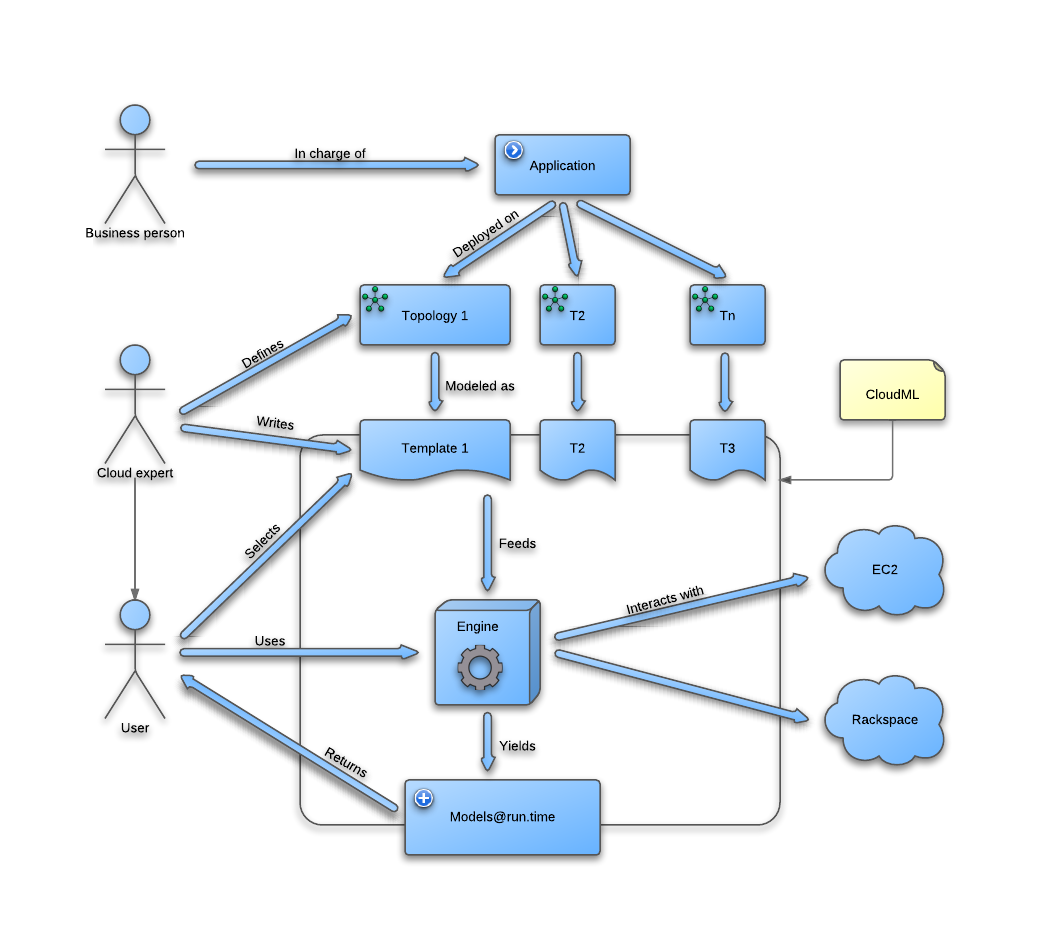
\includegraphics[width=1.5\linewidth]{img/big-picture.png}}
    \caption{``Big picture'', overview of CloudML procedure flow.}
    \label{fig:big-picture}
  \end{center}
\end{figure}


In this chapter the core idea of CloudML will be presented,
how a procedure of node provisioning is conducted in the perspective of different actors.

The concept and principle of CloudML is to be an easier and more reliable
path into cloud computing for IT-driven businesses of variable sizes.
The tool is visioned to parse and execute template files representing topologies
of instances in the cloud. 

\section{The ``big picture''}

The vision of CloudML is reflected through \citefig{big-picture} which gives
an overview of the procedure flow in and around CloudML.

\paragraph{Domain of CloudML.}

Inside \citefig{big-picture} there is an area pointed out as \emph{CloudML},
this area contain components necessary to implement in order to fulfill
the vision as a whole.
Every part within the designated area is some physical aspect in the 
implementation, and therefore core parts of the contribution.

\paragraph{The actors.}

In \citefig{big-picture} there are three actors,
\begin{ii}
  \iitem business person representing someone with administrative or manager position which
    defines and controls demands for application functionality and capabilities.
    The next actor,
  \iitem cloud expert has a greater knowledge of the cloud domain \eg Cloud providers,
    services these offer, limitations, API support and prices.
    The last actor,
  \iitem user is a person which directly utilize CloudML to do provisioning.
    This physical person may or may not have the role of cloud expert, hence 
    the actor extends from cloud expert.
\end{ii}

\paragraph{Application and topologies.}

The business person is in charge of the application, he or she has a need
for an application that can fulfill certain tasks, and to do handle these 
tasks reflecting demands are made.
The cloud expert use the requirements sketched by the business person to 
define and design node topologies which tackles the application demands.
A topology is a map of nodes connected together in a specific pattern, 
defined by the cloud expert.
In a topology there is also information about node attributes 
\eg \myac{CPU} power and \myac{RAM} sizes.
He or she might create several topologies to fulfill the application demands.

\paragraph{Templates.}

The next step is to create templates based on the topologies, this is done by
the cloud expert.
A template is a digital reflection of a topology including the attributes and some additional 
information such as node names and template labeling.
It is also possible to define more than one topology within a single template,
but for the sake of tidiness, clarity and technical limitations it 
should not be possible to define cross-provider (\emph{multicloud}) nodes in a single topology.
This itself does not mean CloudML will not support multicloud provisioning,
instead such functionality is achieved by utilizing more than one template,
which will not retain a full multicloud deployment.

\paragraph{Engine.}

When the cloud expert have designed and created the necessary templates the next actor, 
user, will continue the procedure.
The user select the templates and feed them into the engine.
The engine is the core of the implementation handling several steps and executing
most of the CloudML logic.
The engine operates in five different steps, \
\begin{ii}
  \iitem convert the template files into a native format for later use, 
  \iitem convert pure nodes into instances ready for provisioning, 
  \iitem connect to all the desired providers and 
  \iitem propagate these. Lastly it will produce
  \iitem models@run.time of the nodes being propagated.
\end{ii}

\paragraph{Providers.}

The engine interacts with the providers, in \citefig{big-picture} 
\myac{EC2} and Rackspace are selected as examples, but any
cloud provider that will be supported by CloudML can be utilized.
As discussed in \citechap{state-of-the-art} and \citechap{challenges}
different providers implement different solutions for communication
\eg for provisioning nodes, managing nodes and services or terminating instances.
For engine to interact with a set of different provider some tools, libraries
or framework is needed.

\paragraph{Models@run.time.}

The last part of this implementation of CloudML (see \citechap{perspectives} is to
reflect provisioned instances with models@run.time.
These models are returned to the user when provisioning starts, when
attributes and statuses about instances are updated the user can be 
notified about these updates through the models.
In the implementation the models can extend from or aggregate \emph{instances}.

\mychapter{design}{Analysis and design - CloudML}

In the previous chapter, \citechap{vision}, the core vision of CloudML was presented,
including descriptions of surrounding elements, \eg actors and topologies.
In this chapter the focus is narrowed down to the design and considerations 
of the implementation that constitutes CloudML.

\mysection{meta-model}{Meta-model}
\begin{figure}[tb]
  \begin{center}
      \begin{tikzpicture}[scale=0.6, transform shape]

        \node (UserLibrary) [class] { \textbf{UserLibrary} };

        \node (CloudMLEngine) [class, text width=7cm, rectangle split, rectangle split parts=3, below=of UserLibrary] {
                \textbf{CloudMLEngine}
                \nodepart{second}
                \nodepart{third}
                  +build(a: Account, t: List[Template]): List[RuntimeInstance] \\
                  +status(r: RuntimeInstance, s: Status)
          };

        \node (Account) [class, rectangle split, rectangle split parts=2, 
          left=of CloudMLEngine, xshift=-0cm, label=left:*] {
                \textbf{Account}
                \nodepart{second}+name: String
          };
        \node (Credential) [class, below=of Account, label=67.5:1] { \textbf{Credential} };
        \node (KeyPair) [class, rectangle split, rectangle split parts=2, below=of Credential, xshift=-1cm] {
                \textbf{KeyPair}
                \nodepart{second}+public: String
          };
        \node (Password) [class, rectangle split, rectangle split parts=2, right=of KeyPair] {
                \textbf{Password}
                \nodepart{second}+identity: String \\ +credential: String
          };

        \node (Connector) [class, right=of CloudMLEngine, label=175:*, label=67.5:1] { \textbf{Connector} };
        \node (AmazonEC2) [class, below=of Connector, xshift=-2.5cm, yshift=-.5cm] { \textbf{AmazonEC2} };
        \node (Rackspace) [class, right=of AmazonEC2] { \textbf{Rackspace} };

        \node (Instance) [class, rectangle split, rectangle split parts=2, below=of CloudMLEngine,
          xshift=2cm, yshift=-1cm] { 
          \textbf{Instance} 
          \nodepart{second}templateName: String
        };
        \node (RuntimeInstance) [darkclass, rectangle split, rectangle split parts=3, 
          below=of Instance, xshift=-0cm, label=67.5:*] { 
          \textbf{RuntimeInstance} 
          \nodepart{second}
          \nodepart{third} 
            +update(s: Status) \\
            +getStatus() : Status
        };
        \node (RuntimeProp) [darkclass, left=of RuntimeInstance, label=5:*] { \textbf{RuntimeProp} };
        \node (PublicIP) [darkclass, rectangle split, rectangle split parts=2, below=of RuntimeProp, yshift=-1cm] {
                \textbf{PublicIP}
                \nodepart{second}+value: Address
          };
        \node (Status) [darkclass, rectangle split, rectangle split parts=2, left=of PublicIP] {
                \textbf{Status}
                \nodepart{second}+value: String 
          };
        \node (PrivateIP) [darkclass, rectangle split, rectangle split parts=2, right=of PublicIP] {
                \textbf{PrivateIP}
                \nodepart{second}+value: Address
          };

        \node (Template) [class, rectangle split, rectangle split parts=2, right=of Instance, label=-5:*] {
                \textbf{Template}
                \nodepart{second}+name: String
          };
        \node (Node) [class, rectangle split, rectangle split parts=2, below=of Template, label=67.5:*] {
                \textbf{Node}
                \nodepart{second}+name: String
          };
        \node (Property) [class, below=of Node, label=67.5:*] { \textbf{Property} };
        \node (Location) [class, rectangle split, rectangle split parts=2, below=of Property, yshift=-2cm] {
                \textbf{Location}
                \nodepart{second}+value: String
          };
        \node (Disk) [class, rectangle split, rectangle split parts=2, left=of Location] {
                \textbf{Disk}
                \nodepart{second}+min: String
          };
        \node (Core) [class, rectangle split, rectangle split parts=2, left=of Disk] {
                \textbf{Core}
                \nodepart{second}+min: String
          };
        \node (RAM) [class, rectangle split, rectangle split parts=2, left=of Core] {
                \textbf{RAM}
                \nodepart{second}+min: String
          };

        \draw[extend] (Password) -- ++(0, 1.25) -| (Credential);
        \draw[extend] (KeyPair) -- ++(0, 1.25) -| (Credential);

        \draw[extend] (AmazonEC2) -- ++(0, 0.75) -| (Connector);
        \draw[extend] (Rackspace) -- ++(0, 0.75) -| (Connector);

        \draw[extend] (RAM) -- ++(0, 0.9) -| (Property);
        \draw[extend] (Core) -- ++(0, 0.9) -| (Property);
        \draw[extend] (Disk) -- ++(0, 0.9) -| (Property);
        \draw[extend] (Location) -- ++(0, 0.9) -| (Property);

        \draw[extend] (PublicIP) -- ++(0, 0.9) -| (RuntimeProp);
        \draw[extend] (PrivateIP) -- ++(0, 0.9) -| (RuntimeProp);
        \draw[extend] (Status) -- ++(0, 0.9) -| (RuntimeProp);

        \draw[line] (Account) -- ++(0, 1.5) -| (Connector);

        \draw[aggregate] (UserLibrary) -| (11, -1) -- (11, -6) -| (Template.east);
        \draw[aggregate] (UserLibrary) -| (Account.west);

        \draw[aggregate] (Account) -- (Credential.north);

        \draw[aggregate] (CloudMLEngine.east) -| (Connector.west);

        \draw[aggregate] (Template) -- (Node.north);
        \draw[aggregate] (Node) --  (Property.north);

        \draw[line] (Instance.east) -| ++(0.5, 0) -- ++(0, -2) -| (Node.west);

        \draw[aggregate] (RuntimeInstance.north) -- (Instance);

        \draw[aggregate] (RuntimeInstance) -| (RuntimeProp.east);

    \end{tikzpicture}
  \end{center}
  \caption{Meta model of CloudML.}
  \label{fig:meta-model}
\end{figure}


In this section the meta-model of CloudML will be presented.
The meta-model is visualized in \citefig{meta-model},
and will be described through a specific scenario.
The scenario also describe parts of the implementation design through how it is used.

\paragraph{Scenarios introduction.}

CloudML is introduced by using two different scenarios where a user named \emph{``Alice''} is provisioning the 
\emph{BankManager} application from \citechap{challenges} to the \myac{AWS} cloud.
It is compulsory that she possesses an \myac{AWS} account in advance of the scenario.
This is essential information needed for the scenario to be successful,
and since she is indirectly using \myac{AWS} \myac{API}s,
she must also have \emph{security credentials},
\ie \emph{Access Key ID} and \emph{Secret Access Key}.

The roles assumed by Alice in this scenario, regarding \citefig{big-picture},
are both \emph{cloud expert} and \emph{user}.
She will define the topologies, create the templates and use 
the \emph{engine} to provision her models.
In addition to these roles she is also partly \emph{application designer/developer},
because of tight coupling between running instances and application deployment.

\paragraph{Authentication.}

She associates \emph{Access Key ID} and \emph{Secret Access Key} with 
\texttt{Credential} and \texttt{Password} in \citefig{meta-model}.
\texttt{Credential} is used to authenticate her to supported providers through \texttt{Connector}.
The \texttt{Connector} is a common interface against supported providers.
This component of CloudML is directly associated with \citereq{multi-cloud}.
\texttt{Credential} is in this case in the form of an \texttt{Access Key ID} (random GUID),
but with other providers it might be in another form, \eg a username for Rackspace.
Although the form is different, the physical object type (String) is the same.

\subsection{Single node topology}

Initially Alice is using the topology shown in~\citefig{singlenode}.
This topology introduces a single node, which hosts every tier of the application.
This is not an uncommon topology for development purposes.

\paragraph{Topology considerations.}

Alice establishes a \emph{single-node} based topology, as seen in \citefig{singlenode}.
Since this single node handles both computation and storage, 
Alice decides to increase capabilities of both processing (number of \texttt{Cores}) and 
\texttt{Disk} size on the \texttt{Node}.
Both of these attributes are incremented because the instance hosts
the main application as well as the database.

The approach of using one single node is good in terms of simplicity,
since all important components of the application are located in one single place.
Other advantages distinguish themselves as well, such as network connections where
the address of other components are determined to be \emph{``this computer''} (\emph{localhost}).

\paragraph{Building templates.}

In the end Alice inserts all data about topologies into a \texttt{Template}. 
The template include physical descriptions of the \texttt{Node},
and a list of the type \texttt{Property} for the node.
The \texttt{Node} has a \texttt{name} used to reference the node under provisioning.
The properties the node can have are configurations of attributes on a set of given capabilities.
These configurations are what define what type of tasks a node is suitable for.
In Alice's case the node has increased two important attributes to support both higher computation 
demand and storage capabilities, \ie $2$ cores and $500$ \myac{GB}\footnote{
  Size is expressed in \myac{GB}, but measurement can change depending on implementation of \citereq{software-reuse}.
}
in hard drive size.
By not altering any other attributes on the respective nodes, they will be set to minimal values.
This is a positive expectation, since the nodes will handle specific tasks, which does not 
demand enhancing of other attributes.

\paragraph{Provisioning.}
\begin{figure}
  \begin{center}
    \subfigure[Template with nodes] {
      \begin{tikzpicture}[scale=0.7, transform shape]
        \node (Template) [class, rectangle split, rectangle split parts=2] {
          \textbf{:Template}
          \nodepart{second}name=``template1''
        };
        \node (Node) [class, rectangle split, rectangle split parts=2, right=of Template] {
          \textbf{:Node}
          \nodepart{second}name=``node1'' \\ cores=2 \\ disk=2000
        };

        \draw[line] (Template) -- (Node);
      \end{tikzpicture}
      \label{fig:scenario1-1}
    }
    
    \subfigure[Instance] {
      \begin{tikzpicture}[scale=0.7, transform shape]
        \node (Instance) [class, text width=4.5cm, rectangle split, rectangle split parts=2] {
          \textbf{:Instance}
          \nodepart{second}name=``node1'' \\ cores=2 \\ disk=2000 \\ templateName=``template1''
        };
      \end{tikzpicture}
      \label{fig:scenario1-1}
    }
  \end{center}
  \caption{Object diagram of scenario with one node}
  \label{fig:scenario1}
\end{figure}


\begin{figure}[tb]
  \begin{sequencediagram}
    \newthread{u}{:User}
    \newthreadhack{c}{:CloudML}
    \newinst{r}{r:RuntimeInstance}
    \newthread{a}{:AWS}
    
    \begin{call}{u}{build(\texttt{account},List(\texttt{template}))}{c}{List(\texttt{r})}
      \begin{call}{c}{Initialize()}{r}{}
      \end{call}
    \end{call}
    \begin{messcall}{c}{provision(\texttt{r})}{a}
    \end{messcall}
    
    \begin{call}{u}{getStatus()}{r}{\emph{"Building"}}
    \end{call}
    
    \begin{messcall}{a}{status(\texttt{r}, \emph{"Starting"})}{c}
    \end{messcall}
    
    \begin{messcall}{c}{update(\emph{"Starting"})}{r}
    \end{messcall}
    
    
    \begin{call}{u}{getStatus()}{r}{\emph{"Starting"}}
    \end{call}
  \end{sequencediagram}
  
  \caption{CloudML asynchronous provisionning process (Sequence diagram).}
  \label{fig:sequence-singlenode}
\end{figure}


With these models Alice initializes provisioning by calling 
\texttt{build} on \texttt{CloudMLEngine}, providing \texttt{Credential} and \texttt{Template}.
This starts the asynchronous job of configuring and creating 
\texttt{Instances} based on \texttt{Nodes}.
In \citefig{scenario1-1} an object diagram describe the initial configuration at run-time,
after CloudML has interpreted the templates.
The instance produced by the template and node is in the form of a single object,
as represented by the object diagram in \citefig{scenario1-2}.
\texttt{Instance} only refer to template by a \emph{String}, \texttt{templateName}.
This is semantically correct because the template is a transparent entity
in the context of provisioning, and is only used as a reference.
\texttt{Instance} is also an \emph{internal} element in CloudML, and might not 
have to be indirectly or directly exposed to end users.

\texttt{RuntimeInstance} is specifically designed to complement \texttt{Node} with \texttt{RuntimeProperties},
as \texttt{Properties} from \texttt{Node} still contain valid data.
When \texttt{CloudMLEngine} start provisioning, a \texttt{RuntimeInstance} is created immediately,
and returned to Alice.
These are \myac{M@RT} within CloudML, designed to provide asynchronous provisioning
according to \citereq{m@rt}.
They are reflections of \texttt{Instance}, and they aggregate instances.

The method call to \texttt{build} is described in \citefig{sequence-singlenode}.
In this figure \texttt{RuntimeInstance} is returned directly to Alice,
because these are asynchronous elements within CloudML, which end users can gather 
information through.
The actor \texttt{CC} within this figure is an abbrevation of \texttt{CloudConnector}.
This is emphasized within \citefig{sequence-singlenode} through \texttt{getStatus} method calls.
\texttt{Instance} is never visualized, this is because it is an internal format
within CloudML and does not need to be presented in the sequence diagram,

When the \texttt{Node} is provisioned successfully and sufficient meta-data is gathered,
Alice can start the deployment.
CloudML has then completed its scoped task of provisioning.

\subsection{Three nodes topology}

For scalability and modularity the \emph{single-node} approach is restraining,
\ie it does not scale very well, and does not benefit from cloud advantages.
If the application consumes too much \myac{CPU} power, 
this slows the application totality down and decreases usability.
There is no strong link between CloudML and the application, but to maintain
scalability some measures must be manually developed into \emph{BankManager}.
So the initial application code includes support for work load distribution through 
application design and deployment considerations.
In \emph{BankManager} these measures consists of manually setting 
physical database address before deploying the application.

In the previous described scenario, 
Alice provision \emph{BankManager} to one single instance on \myac{AWS}.
This setup is sufficient for development purposes, but major advantages
could be gained through the opportunity of horizontal scalability (\emph{scale out}).
There are distinct benefits to this.
If Alice deployed an application that should suddenly, 
rapidly and unexpectedly gain popularity, her current setup (one single node) will not be sufficient.
In case of such event Alice should change her topology from her initial one seen in 
\citefig{singlenode} with one node, to that of \citefig{threenodes} with three nodes.
Or even the topology seen in \citefig{frontends}, with \emph{``unlimited''} amount of nodes.
This topology is more advanced and utilizes the cloud on a higher level.
It has three nodes, two for the application logic (front-end) and one for the database (back-end).
In front it has a \emph{load balancer}, which is a cloud service ensuring that requests
are spread between front-end nodes based on predefined rules.
Even though this service is meant for balancing requests to front-ends,
it can actually be used internally in between local nodes as well.

\paragraph{New template.}

Alice changes her topology by editing her existing \texttt{Template} 
to contain three nodes instead of one. 
She also changes the node attributes to suite their new needs better,
\ie increasing amount of \texttt{Cores} on front-end, and increased \texttt{Disk} for back-end \texttt{Node}.
The characteristics Alice choose for her \texttt{Nodes} and \texttt{Properties} are fitted
for the chosen topology.
All \texttt{Properties} are optional and thus Alice does not have to define them all.

\paragraph{Rebuild.}
\begin{figure}[th]
  \hspace*{-2cm}
  \begin{sequencediagram}
    \newthread{u}{:User}
    \newthreadhack{c}{:CloudML}
    \newinst{r1}{r1}
    \newinst{r2}{r2}
    \newinst{r3}{r3}
    \newthread{a}{:AWS}
    
    \begin{call}{u}{build(\texttt{account},List(\texttt{template}))}{c}{
        List(\texttt{r1}, \texttt{r2}, \texttt{r3})}
      \begin{call}{c}{Initialize()}{r1}{}
      \end{call}
      \begin{call}{c}{Initialize()}{r2}{}
      \end{call}
      \begin{call}{c}{Initialize()}{r3}{}
      \end{call}
    \end{call}

    %\begin{messcall}{c}{provision(\texttt{r1})}{a}
    %\end{messcall}
    %\begin{messcall}{c}{provision(\texttt{r2})}{a}
    %\end{messcall}
    %\begin{messcall}{c}{provision(\texttt{r3})}{a}
    %\end{messcall}
    \begin{messcall}{c}{provision nodes(\texttt{r1}, \texttt{r2}, \texttt{r3})}{a}
    \end{messcall}
    
    \begin{call}{u}{getStatus()}{r1}{\emph{"Building"}}
    \end{call}
    \begin{call}{u}{getStatus()}{r2}{\emph{"Building"}}
    \end{call}
    
    \begin{messcall}{a}{status(\texttt{r1}, \emph{"Starting"})}{c}
    \end{messcall}
    \begin{messcall}{c}{update(\emph{"Starting"})}{r1}
    \end{messcall}
    
    
    \begin{call}{u}{getStatus()}{r1}{\emph{"Starting"}}
    \end{call}
    \begin{call}{u}{getStatus()}{r2}{\emph{"Building"}}
    \end{call}

    \begin{messcall}{a}{status(\texttt{r1}, \emph{"Started"})}{c}
    \end{messcall}
    \begin{messcall}{c}{update(\emph{"Started"})}{r1}
    \end{messcall}
    \begin{messcall}{a}{status(\texttt{r2}, \emph{"Starting"})}{c}
    \end{messcall}
    \begin{messcall}{c}{update(\emph{"Starting"})}{r2}
    \end{messcall}

    \begin{call}{u}{getStatus()}{r1}{\emph{"Started"}}
    \end{call}
    \begin{call}{u}{getStatus()}{r2}{\emph{"Starting"}}
    \end{call}
    \begin{call}{u}{getStatus()}{r3}{\emph{"Building"}}
    \end{call}
  \end{sequencediagram}
  
  \caption{CloudML asynchronous provisionning process (Sequence diagram).}
  \label{fig:sequence-threenodes}
\end{figure}


Then she executes \texttt{build} on \texttt{CloudMLEngine} again,
which will provision the new nodes for her.
She will get three new nodes, and the previous provisioned nodes must be manually terminated
(more about this in \citechap{perspectives}).
The outline of how nodes are provisioned is shown in \citefig{sequence-threenodes-1}.
The asynchronous behavior is expressed in \citefig{sequence-threenodes-2}.
This behavior is similar to that shown in \citefig{sequence-singlenode},
but show how communication can flow with increased amount of \texttt{RuntimeInstances}.
In the figure \texttt{RI} is an abbreviation of \texttt{RuntimeInstance}, to save space.
For the same purpose, \texttt{CC} is an abbreviation of \texttt{CloudConnector}.
It is also split into three parts expressing different steps, 
\begin{ii}
  \iitem provisioning, 
  \iitem node communications and
  \iitem how a load balancer service is established.
\end{ii}
This figure is similar to \citefig{sequence-singlenode}, but with three nodes instead of one.
Both percept \iii{1} and \iii{2} are found in \citefig{sequence-singlenode}.
Another difference is that \texttt{User} does more calls to \texttt{CloudML},
which express how statuses between \texttt{RI}s are updating.

When connecting front-end instances of \emph{BankManager} to back-end instances Alice must 
be aware of the back-ends \texttt{PrivateIP} address, which she will retrieve from CloudML
during provisioning according to \myac{M@RT} approach.
This was not necessary for the initial scenario setup, but could still be applied
as good practice.

\paragraph{Three nodes summary.}
\begin{figure}[tb]
  \begin{center}
    \subfigure[Template with nodes] {
      \begin{tikzpicture}[scale=0.7, transform shape]
        \node (Template) [class, rectangle split, rectangle split parts=2] {
          \textbf{:Template}
          \nodepart{second}name=``template1''
        };
        \node (Node02) [class, rectangle split, rectangle split parts=2, right=of Template] {
          \textbf{:Node}
          \nodepart{second}name=``node2'' \\ cores=2
        };
        \node (Node01) [class, rectangle split, rectangle split parts=2, above=of Node02] {
          \textbf{:Node}
          \nodepart{second}name=``node1'' \\ cores=2
        };
        \node (Node03) [class, rectangle split, rectangle split parts=2, below=of Node02] {
          \textbf{test1:Node}
          \nodepart{second}name=``node3'' \\ disk=2000
        };

        \draw[line] (Template) -- (Node01);
        \draw[line] (Template) -- (Node02);
        \draw[line] (Template) -- (Node03);
      \end{tikzpicture}
      \label{fig:scenario2-1}
    }

    \subfigure[Instance] {
      \begin{tikzpicture}[scale=0.7, transform shape]
        \node (Instance01) [class, text width=4.5cm, rectangle split, rectangle split parts=2] {
          \textbf{:Instance}
          \nodepart{second}name=``node1'' \\ cores=2 \\ templateName=``template1''
        };
        \node (Instance02) [class, text width=4.5cm, rectangle split, rectangle split parts=2, right=of Instance01] {
          \textbf{:Instance}
          \nodepart{second}name=``node2'' \\ cores=2 \\ templateName=``template1''
        };
        \node (Instance03) [class, text width=4.5cm, rectangle split, rectangle split parts=2, right=of Instance02] {
          \textbf{:Instance}
          \nodepart{second}name=``node4'' \\ disk=2000 \\ templateName=``template1''
        };
      \end{tikzpicture}
      \label{fig:scenario2-2}
    }
  \end{center}
  \caption{Scenario reimplemented with three nodes.}
  \label{fig:scenario2}
\end{figure}



The benefits of a topology where the application is distributed over several nodes 
is the scalability and modularity, which were lacking in the \emph{single-node} topology.
For instance, if the user demand should rapidly increase, Alice could change her topology to
provision more front-end nodes as seen in \citefig{frontends}.
This could be done presumably without greater changes to origin application,
since the application is initially designed for such a distributed topology.

An object diagram of the topology is shown in \citefig{scenario2-1}.
There is nothing that concretely separate front-end nodes from back-end nodes,
this can only be determined from node \texttt{name} or what attributes are altered.
The separation is completely up to Alice when doing the deployment,
\ie nothing in CloudML will restrain or limit Alice 
when it comes to work load distribution between nodes.

As with the instances in \citefig{scenario1-2} the instances in \citefig{scenario2-2}
are reflections of the nodes (and template) in \citefig{scenario2-1}.
The template name is referenced within each \texttt{Instance} 
for the reasons mentioned earlier.

\subsection{Multi-cloud provisioning}

Alice could later decide to use another provider, either as replacement or complement to her current setup,
because of availability, financial benefits or support.
To do this she must change the provider name in \texttt{Account} and call \texttt{build} on \texttt{CloudMLEngine} again,
this will result in an identical topological setup on a supported provider.
\texttt{UserLibrary} in \citefig{meta-model} visualizes that \texttt{Account} and \texttt{Template} are 
physical parts maintainable by the user.

The \texttt{build} method support provisioning of several templates to one account (same provider).
There is also a constraint/limitation, a set of templates can not be simultaneously 
cross-deployed to different providers,
\ie not possible to define cross-provider (\emph{multi-cloud}) nodes in a single topology.
This is for the sake of tidiness, clarity and technical limitations.
CloudML support multi-cloud provisioning,
just that such functionality is achieved by sequential re-provisioning,
which will not retain a full multi-cloud deployment.

\paragraph{\myac{AWS} and Rackspace combined.}
\begin{figure}[tb]
  \tikzstyle{browser}=[rectangle, dashed, draw=black, rounded corners, fill=white!40, drop shadow,
  text centered, anchor=north, text=black, text width=3.5cm, top color=white, bottom color=black!10]

  \begin{center}
      \begin{tikzpicture}[scale=.7, transform shape]

        \node (Browser) [browser, text width=1.5cm] { \textbf{Browser} };

        \node (AWS) [rectangle, draw, rounded corners, right of=Browser, label=below:AWS,
          minimum width=12cm, minimum height=5cm, xshift=9cm, yshift=0cm] {};

        \node (LoadBalancer) [tdiamond, right=of Browser] { \textbf{Load balancer} };
        \topologyntimes{right=of LoadBalancer}{Frontend}{Front-end}
        \node (Backend) [class, right=of Frontend-1, yshift=-1cm] { \textbf{Back-end} };

        \node (Backend-master) [class, below=of Backend, yshift=-5cm] { \textbf{Back-end master} };

        \node (Rackspace) [rectangle, draw, rounded corners, left of=Backend-master, 
          minimum width=12cm, minimum height=5cm, xshift=-2.5cm, label=below:Rackspace] {};

        \topologyntimes{left=of Backend-master}{Slave}{Slave}

        \draw[extend] (Browser.east) -- (LoadBalancer.west);
        \draw[extend] (LoadBalancer.east) -- (Frontend-1.west);
        \draw[extend] (LoadBalancer.east) -- (Frontend-2.west);
        \draw[extend] (LoadBalancer.east) -- (Frontend-n.west);
        \draw[extend] (Frontend-1.east) -- (Backend.west);
        \draw[extend] (Frontend-2.east) -- (Backend.west);
        \draw[extend] (Frontend-n.east) -- (Backend.west);

        \draw[extend] (Backend) -- (Backend-master);
        \draw[extend] (Backend-master.west) -- (Slave-1.east);
        \draw[extend] (Backend-master.west) -- (Slave-2.east);
        \draw[extend] (Backend-master.west) -- (Slave-n.east);
      \end{tikzpicture}
  \end{center}

  \caption{Multicloud topology.}
  \label{fig:topology-multicloud}
\end{figure}


To describe the layout of a multi-cloud provisioning with CloudML,
a scenario is invented and a complementary figure is crafted.
In the new scenario Alice creates a topology spanning over two providers,
as seen in \citefig{topology-multi-cloud}.
In the figure the user connects to a \texttt{load balancer}, 
then the request is distributed between a set of \texttt{front-ends} which will 
retrieve appropriate data from a \texttt{back-end}.
This is similar to \citefig{threenodes} with three nodes.
Everything so far is under the realm of \myac{AWS},
including a \texttt{load balancer}, $n$ amount of nodes for \texttt{front-end} computation
and one \texttt{back-end} node.
In this case the \texttt{back-end} does not hold any data, instead it is connected
to another node \emph{cross provider} to Rackspace.
On Rackspace a set of nodes are built to hold data,
one \texttt{back-end master} manages a set of $n$ \texttt{slaves}.
The \texttt{slave} nodes hold all data.

\mysection{technological-assessments}{Technological assessments and considerations}

\subsection{Programming language and application environment.}

When considering \emph{programming language} and \emph{application environment} 
the important aspects are the ones mentioned in \citereq{foundation},
\begin{ii}
  \iitem ease of use,
  \iitem community size,
  \iitem closed/open source,
  \iitem business viability,
  \iitem modernity and 
  \iitem matureness.
\end{ii}
For the implementation to be a successful approach towards CloudML 
the aspects chosen must also be relevant for future improvements.
At the same time the aspects chosen must be appealing to existing communities of interest,
without this it will not gain the footing it needs.
The most important aspects are therefore precept \iii{2}, \iii{5} and \iii{6}.

\subsection{Asynchronous information gathering and distribution.}

\paragraph{The design.}

When a node is being propagated it changes type from \texttt{Instance} to 
\texttt{RuntimeInstance}, which can have a different \emph{state} such as 
\emph{Configuring}, \emph{Building}, \emph{Starting} and \emph{Started}.
Considerations for implementation are described in \citesec{modules}.

When a \texttt{RuntimeInstance} reaches \emph{Starting} state the provider 
has guaranteed its existence, including the most necessary metadata.
When all nodes reaches this state the task of provisioning is concluded.

\paragraph{Patterns.}

Provisioning nodes is by its nature an asynchronous action that can take minutes to execute.
For CloudML to compensate with this asynchronous behavior several approaches could be made,
as mentioned in \citechap{requirements}, \ie observer pattern, command pattern, actor model,
or publish-subscribe pattern.
Patterns tightly bound to using an object-oriented language for \citereq{foundation}.
The core idea of integration and benefits of these approaches are:
\begin{description}
  \item[Observer pattern.] The essence of this pattern is a one-to-many distribution of events between objects.
    This can be explained with a restaurant as an example, with one chef and two waiters.
    The chef is an \emph{observable} and the two waiters are \emph{observers}.
    The chef does some work (cooking), and when he or she is complete with a dish all observers are notified.
    The observers receive this event and can act upon it, 
    \eg the first waiter ignores the dish, because it does not belong to any of his or her tables, 
    while the other waiter takes the dish to appropriate table.
  \item[Command pattern.] Is about encapsulating data and logic. 
    Implementations have a known method, \eg \emph{execute} which comes from an \emph{interface}.
    So logic could be transparent when invoking them.
    In the restaurant-example one can consider a general \emph{waiter} to be the interface,
    and the two waiters would each be separate implementations, 
    \eg \emph{TableAToC} and \emph{TableDToH}.
    When the chef \emph{invokes} the method \emph{execute} on any type of \emph{waiter}, 
    he or she does not need to know anything about their implementation, 
    each waiter will know by themselves which table to visit.
  \item[Actor model.] Solves the problem with asynchronous communication through passing messages
    in between \emph{actors}.
    These messages are decoupled from the sender, resulting in proper asynchronous communication.
    Actors can also create new actors.
    With the restaurant-example one can imagine all three elements, \ie chef, first and second waiter,
    to be individual actors.
    The chef must know about the first waiter, 
    but the waiters do not necessarily need to know about each other.
    When a meal is done the chef can inform the correct waiter 
    (the one associated with the correct table).
    The benefit here is that the message is decoupled and asynchronous, so the chef can start
    working on the next meal without waiting for the waiter to return.
  \item[Publish-subscribe pattern.] This pattern is very similar to observer pattern in behavior,
    but is more focused on message distribution logic.
    Compared to observer pattern the \emph{observable} are considered a \emph{publisher} and
    \emph{observers} are called \emph{subscribers}.
    When a \emph{publisher} sends a message it does not send it directly to any receivers,
    instead there is a filter-based logic which selects receivers based on condition they set themselves.
    In the restaurant example, similar to that with observer pattern, the chef is \emph{publisher}
    and both waiters are \emph{subscribers}.
    When the chef completes a meal he or she notify the waiters based on their \emph{conditions},
    \eg the first waiter listen for events of type \emph{TableA}, \emph{TableB} and \emph{TableC}.
    If the finished meal was assigned for table $A$ the first waiter would get the message.
\end{description}
Of these solutions the most promising one is \emph{actor model} because it is more directly aimed
at solving asynchronous communication.
The other solutions can provide assistance by accommodating communications through events, 
but by them selves they do not solve the issue of slow provisioning.
An interesting approach is to combine the \emph{actor model} with one of the patterns.
By doing this the behavior functionality is combined with the asynchronous benefits within the actor model.
Of the previous mentioned patterns only \emph{observer} and \emph{publish-subscribe} patterns 
fit well with designed behavior of CloudML.
Of these \emph{publish-subscribe} is the most scalable and dynamic one (at run-time),
but also the most complicated.
When combining the \emph{actor model} with such pattern it is important to keep the implementation
as simple as possible, without withholding functionality.
Hence the best solution for CloudML is to combine \emph{actor model} with \emph{observer pattern}.

The \emph{actor model} can be implemented in many different ways, even on different tiers.
Both requirement \citereq{foundation} and \citereq{software-reuse} can assist with either
a built-in functionality in the language, environment or an external library or framework.
The observer pattern can be implemented in many ways,
\eg using \texttt{java.util.Observer} and \texttt{java.util.Observable}.

\subsection{Lexical format.}

Requirement \citereq{lexical-template} from \citechap{requirements} consists of two
important core elements.
The first is \emph{important aspect}, \ie functional demands the format must fulfill,
such as how popular it is and how well it is supported by programming languages.
Second element is that of \emph{data format}, \ie the actual language used to 
serialize data.
This last element is not important for design, and will be introduced and
further described in \citesec{technologies} (\citechap{implementation}).
The important aspects of a lexical format for CloudML are:
\begin{itemize}
  \item Renowned among software developer communities, industry and the academic domain.
    The language will be used directly by these parties, so it is beneficial
    that they are familiar with the syntax.
  \item Integrates (supporting libraries) with most common existing technologies.
    The range of \citereq{foundation} should not be limited by the format.
  \item Human-readable, to some extent.
    End users needs to create and edit these files, often by hand.
    Therefore it must be readable and manually maintainable.
  \item Function with web-services and web-based technologies.
    CloudML is a language designed for \emph{cloud environments},
    so choosing a format that works well on the web is crucial.
\end{itemize}

\mysection{modules}{Modules and application flow}

CloudML is divided into four main modules~(\citefig{cloudml-modules}).
This is to distribute workload and divide CloudML into logical parts for different tasks.

\paragraph{Engine.} 

\begin{figure}[tb]
  \begin{center}
    \subfigure[Application module dependencies.]{
      \begin{tikzpicture}[scale=0.8, transform shape]
        \node (AuxNode01) [text width=4cm] {};
        \node (Engine) [class, left=of AuxNode01, rectangle split, rectangle split parts=2] { 
          \textbf{Engine} 
          \nodepart{second}Entry point. Orchestration.
        };
        \node (AuxNode02) [left=of Engine] {};
        \node (Kernel) [class, below=of AuxNode01, rectangle split, rectangle split parts=2] { 
          \textbf{Kernel} 
          \nodepart{second}Node domains. Converts JSON to Node Entities.
        };
        \node (Repository) [class, above=of AuxNode01, rectangle split, rectangle split parts=2] { 
          \textbf{Repository} 
          \nodepart{second}Instance domains. Convert Nodes to Instances.
        };
        \node (Cloud-connector) [class, right=of AuxNode01, rectangle split, rectangle split parts=2] { 
          \textbf{Cloud-connector} 
          \nodepart{second}Connects to providers (jclouds).
        };

        \draw [arrow] (Engine) -- (Kernel);
        \draw [arrow] (Engine) -- (Cloud-connector);
        \draw [arrow] (Engine) -- (Repository);
        \draw [arrow] (Cloud-connector) -- (Kernel.east);
        \draw [arrow] (Cloud-connector) -- (Repository.east);
        \draw [arrow] (Repository) -- (Kernel);
        \draw [extend] (AuxNode02) -- (Engine);
      \end{tikzpicture}
      \label{fig:cloudml-modules-dependencies}
    }

    \subfigure[Application module orchestration/flow. 
      The numbers indicate order of sequential flow.]{
      \begin{tikzpicture}[scale=0.8, transform shape]
        \node (Engine) [class] { \textbf{Engine} };
        \node (Kernel) [class, below=of Engine] { \textbf{Kernel} };
        \node (Repository) [class, above=of Engine] { \textbf{Repository} };
        \node (Cloud-connector) [class, right=of Engine] { \textbf{Cloud-connector} };
        \node (AuxNode01) [left=of Engine] {};

        \draw [arrow, <->] (Engine) -- node[right] {2} (Kernel);
        \draw [arrow, <->] (Engine) -- node[right] {3} (Repository);
        \draw [arrow, <->] (Engine) -- node[above] {4} (Cloud-connector);
        \draw [extend, <->] (AuxNode01) -- node[above]{1} node[below]{5} (Engine);
      \end{tikzpicture}
      \label{fig:cloudml-modules-orchestration}
    }

    \subfigure[Legend.]{
      \begin{tikzpicture}[scale=0.7, transform shape]
        \node (Module) [class, label=below:Application modules] { Module };

        \node (AuxNode01) [right=of Module] {};
        \node (AuxNode02) [right=of AuxNode01] {};
        \node (AuxNode03) [right=of AuxNode02] {};
        \node (AuxNode04) [right=of AuxNode03] {};

        \draw[arrow] (AuxNode01) -- node[below] {Dependency} (AuxNode02);
        \draw[extend] (AuxNode03) -- node[below] {Entry} (AuxNode04);
      \end{tikzpicture}
    }
  \end{center}
  \caption{Modules in CloudML, dependencies and orchestration.}
  \label{fig:cloudml-modules}
\end{figure}

\begin{figure}[tb]

  \begin{center}
    \begin{tikzpicture}
      \stickman{User}{User}

      \node[box, right=of User, minimum width=3.8cm, minimum height=3.5cm, xshift=1cm, yshift=-1cm,
        label=below:CloudML] (System) {};
      \node[box, right=of User, xshift=2cm, yshift=-0cm] (Engine) {Engine};
      \node[box, below=of Engine, yshift=0.5cm] (Cloud-connector) {Cloud-connector};
      \node[box, below=of Cloud-connector, yshift=0.5cm] (RuntimeInstance) {RuntimeInstance};

      \node (Rackspace) [tcloud, right=of System, xshift=0.5cm, yshift=1.5cm] {Rackspace};
      \node (EC2) [tcloud, below=of Rackspace, label=below:Cloud providers] {EC2};

      \draw[arrow] (User.east) -- (Engine.west);
      \draw[arrow] (Engine.south) -| ($(Cloud-connector.north) + (0, .1cm)$);

      \draw[arrow] ($(Cloud-connector.east) + (.1cm, 0)$) -- (Rackspace.west);
      \draw[arrow] ($(Cloud-connector.east) + (.1cm, 0)$) -- (EC2.west);

      \draw[arrow] (Cloud-connector.south) -| ($(RuntimeInstance.north) + (0, .1cm)$);
      \draw[arrow] (RuntimeInstance.west) -- (User.east);
    \end{tikzpicture}
  \end{center}
  \caption{Usage flow in CloudML.}
  \label{fig:cloudml-modules-flow}
\end{figure}


The main entry point to the application is \texttt{Engine}. 
This means it does not have to be initialized and there exists only one instance of it.
Interaction between \texttt{user} and \texttt{Engine} is expressed in \citefig{cloudml-modules-flow} 
where the user will initialize provisioning by calling \texttt{Engine}.
\texttt{Engine} will also do orchestration between the three other modules
as shown in \citefig{cloudml-modules-orchestration}.
Since \texttt{Cloud-connector} is managed by \texttt{Engine},
other actions run against instances are done through \texttt{Engine}.
The first versions of \emph{cloudml-modules} did not use \texttt{Engine} as orchestrator but
instead relied on each module to be a sequential step, this proved to be harder to maintain
and also introduced cyclic dependencies.
\texttt{Engine} has dependencies to all the other modules,
as expressed in \citefig{cloudml-modules-dependencies}.

\paragraph{Kernel.} 

CloudML specific entities are kept in \texttt{Kernel},
such as \texttt{Node} and \texttt{Template}.
This is some of the core parts of the \myac{DSL}, hence it is called \emph{\texttt{Kernel}}.
The logical task of \texttt{Kernel} is to map \myac{JSON} formatted strings to 
\texttt{Templates} including \texttt{Nodes}.
\texttt{Accounts} are separate parts that are parsed equally as \texttt{Templates},
 but by another method call. All this is transparent for users as all data will
be provided directly to \texttt{Engine} which will handle the task
of calling \texttt{Kernel} correctly.
In \citefig{cloudml-modules-dependencies} is it shown that \texttt{Kernel}
has no dependency to other modules, while all the other modules depend on \texttt{Kernel}.
This stresses the fact that \texttt{Kernel} is the most fundamental part,
closest to the \myac{DSL}.
According to \citefig{cloudml-modules-orchestration} \texttt{Kernel} is the first module
to be called by \texttt{Engine}, as it will convert incoming text (\emph{String})
to internal format of \texttt{Nodes}.

\paragraph{Repository.} 

\texttt{Instance} are entities within \texttt{Repository},
these are equivalent to \texttt{Nodes} in \texttt{Kernel},
but are specific for provisioning.
Repository will do a mapping from \emph{Nodes} (including \emph{Template})
to \emph{Instances}. Future versions of \texttt{Repository} will also do some logical superficial validation
against \emph{Node} properties.
At the writing moment (\date{April 2012}) it is not possible to 
demand load balancers (as a service) on Rackspace for specific geographical locations.

\paragraph{Cloud-connector.}

The connections to providers are established through the module \texttt{Cloud-connector}.
This module uses an external software allowing CloudML to connect to several providers
through a common interface.
This software fulfills \citereq{software-reuse}.
The connections to providers are expressed in \citefig{cloudml-modules-flow}.
As expressed in \citefig{cloudml-modules-dependencies} \texttt{Cloud-connector}
depend on both \texttt{Kernel} and \texttt{Repository}.
These dependencies match its task, as it must have knowledge about both 
\texttt{Templates} and \texttt{RuntimeInstance}.
This module is the last step before returning to the user, as seen in \citefig{cloudml-modules-orchestration}.
In \citefig{cloudml-modules-flow} it is expressed that \texttt{Cloud-connector} initializes
the actors (\texttt{RuntimeInstance}) which are provided to the \texttt{User}.

\mychapter{implementation}{Implementation/realization: The cloudml-engine library}

In the previous chapter the design of CloudML was introduced.
In this chapter the implementation of this design will be presented and described.
First section is a technical overview of some of the general solutions within 
the implementation.
The rest of the chapter is split into different sections, one for each important part of the implementation.
Topics are about
\begin{ii}
  \iitem sub-modules and their tasks,
  \iitem the dependency system,
  \iitem communication with cloud providers,
  \iitem \myac{M@RT} through actor model and
  \iitem data serialization.
\end{ii}

\mysection{technologies}{Technology overview}

CloudML is implemented as a \emph{proof-of-concept} framework~\cite{cloudml-engine}
(from here known as \emph{cloudml-engine}). 
The implementation, \emph{cloudml-engine}, 
is based on \emph{state-of-the-art} technologies that appeal to the academic community.
Technologies chosen for \emph{cloudml-engine} are not of great importance to the concept of CloudML itself,
but it is still important to understand which technologies are chosen, what close alternatives exists
and why they are chosen.

\paragraph{Language and environment.} 

The importance of a \emph{programming language} and \emph{environment} were
described in \citesec{technological-assessments}.
These are core ideas to fulfill \citereq{foundation}, emphasizing the importance of a strong foundation.
Here is a list describing some of the languages and environments considered:
\begin{itemize}
  \item Java (\myac{JVM})
  \item JavaScript (Node.js)
  \item Scala (\myac{JVM})
  \item Python
  \item C\# (.NET)
\end{itemize}
Languages in this list are introduced because of their overall popularity.
Some were introduced despite this, such as \emph{Node.js}, 
which is brought in as an consideration because of the abilities to operate
with \myac{JSON}, cloud interaction and modernity.

Based on these considerations Scala is a good choice, it fulfills the core ideas and match
the requirement \citereq{foundation}:
\begin{description} 
  \item[Ease of use.]
    Scala is a \emph{state-of-the-art} language with many technological advantages,
    \eg supporting both functional and object-oriented programming.
    With both paradigms, imperative programmers such as Java developers as well as functional
    programmers such as Clojure developers would be familiar with the language design.
    
    This language emphasizes on functional programming which is leveraged in the implementation.
    Scala has a built in system for actor model~\cite{actors:haller07}, 
    which is utilized in the implementation.
    This also assists in relation to \citereq{m@rt}.

    \myac{JVM} is a popular platform, as the main platform for Java.
    Scala runs on the \myac{JVM}, and support all the libraries and work put into Java
    over the years can be utilized directly by Scala.
  \item[Community size.]
    This language is gaining popularity among both the academic and enterprise domain.
  \item[Closed/open source.] Scala is open source.
  \item[Modernity.]
    The reason not to use plain Java is because Scala is an appealing \emph{state-of-the-art} language.
    The language is under constant development and new features and enhancements keeps improving
    the language.
  \item[Matureness.]
    Compatible with Java and libraries written in Scala can be interacted with by Java as well.
    This means that even though Scala is chosen for the implementation of CloudML,
    it can still be used by other languages supported by the \myac{JVM},
    \eg Java, Groovy and Clojure.
\end{description}
Based on these benefits Scala is chosen, and \emph{cloudml-engine} is written in this language.


\mysection{dependencies}{Automatic build system}
\begin{figure}[tb]
  \subfigure[dependency-graph-without-test] {
    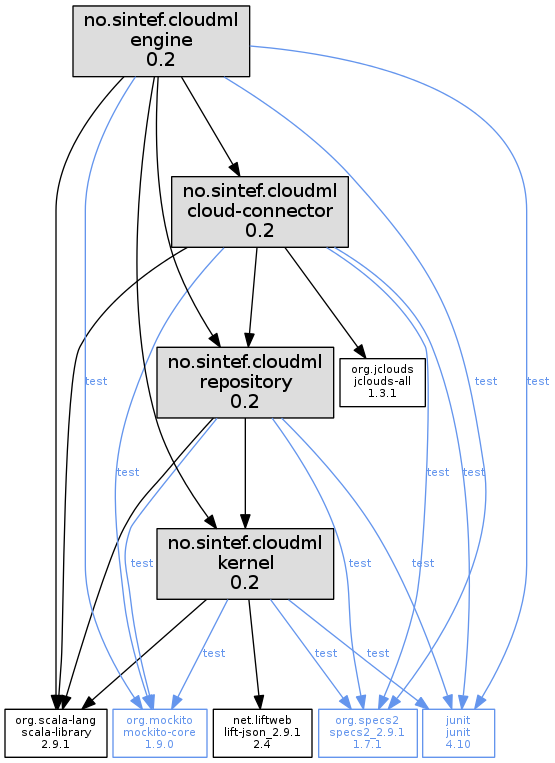
\includegraphics[width=8cm]{imgs/dependency-graph-2.png}
    \label{fig:dependency-graph-without-test}
  }
  \subfigure[dependency-graph-with-test] {
    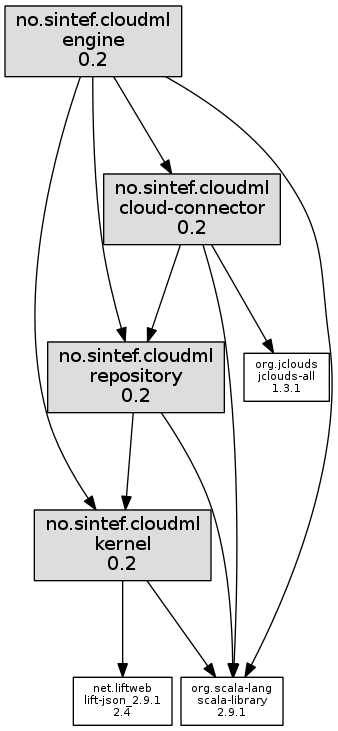
\includegraphics[width=5cm]{imgs/dependency-graph-1.png}
    \label{fig:dependency-graph-with-test}
  }
  \caption{Maven dependency graph (with and without test scope).}
  \label{fig:dependency-graph}
\end{figure}


%this is a \emph{Scala Object} used to initialize provisioning.
%A \emph{Scala Object} works as a \emph{singleton}, 

There are two main methods used to automatically build Scala programs, 
either using a Scala-specific tool called \myac{SBT} or a more general tool called Maven. 
For \emph{cloudml-engine} to have an academic appeal it is essential to choose the technology
with most closeness to Java, hence Maven is the best option.
It is also important to make the library available for developers using Java or other
languages supported by the \myac{JVM}.
This is best achieved by using Maven, as \myac{SBT} is directed at Scala.

In \citesec{modules} CloudML were split into four different modules, as seen in \citefig{cloudml-modules}.
Maven support modules, these are used to split \emph{cloudml-engine} into the appropriate 
modules.

A full Maven dependency graph is expressed in \citefig{dependency-graph}.
There are two graphs, both of \emph{cloudml-engine}.
The first graph~(\citefig{dependency-graph-without-test}) excludes the \emph{test-scope},
while~\citefig{dependency-graph-with-test} includes it.
The \emph{test-scope} is a Maven scope which marks the dependencies to only be included
when running a specific \emph{goal}, \eg test.
In this graph the internal and external dependencies in \emph{cloudml-engine} are expressed.
All external dependencies, 
\eg \texttt{org.jclouds.jclouds-all}~(\citefig{dependency-graph}),
contain even more dependencies to other libraries and internal modules.
These dependencies are all omitted in both graphs.

%The dependencies are defined in \emph{pom.xml}-files.
%Parts of a dependency reference in a Maven configuration can be seen in~\citefig{pom-example},
%although this is not dependency management in between \emph{cloudml-engine} modules but rather
%how to add \emph{cloudml-engine} as a dependency itself.

\section{Cloud connection}
\begin{figure}[tb]
  \begin{center}
    \begin{minted}[mathescape,
                   linenos,
                   numbersep=5pt,
                   frame=lines,
                   framesep=2mm]{scala}
trait CloudConnector {
  def createInstances(template: Template): 
      List[RuntimeInstance]
  def destroyInstance(id: String)
}
object CloudConnector {
  def apply(account: Account, instanceType: String): 
      CloudConnector = instanceType match {
    case "jclouds" =>
      new JcloudsConnector(account);
    case _ =>
      new JcloudsConnector(account);
  }
}
    \end{minted}
  \end{center}
  \caption{Facade used in \texttt{cloud-connector}.}
  \label{list:connector-facade}
\end{figure}



The connection between CloudML and cloud providers is facilitated 
through a separate module, called \texttt{cloud-connector}.
In the implementation this module is the bridge between providers and \emph{cloudml-engine}.
It is built to support several libraries and interface these,
this is achieved by implementing a type of \emph{facade pattern}.
It does not contain any entities, and only executes logical code. 

The \emph{facade pattern} used to select which library to use is expressed in
\citelist{connector-facade}.
In this listing an implementation of \texttt{CloudConnector} is returned
based on Scala \emph{pattern matching}.
By default the implementation using \emph{jclouds} is returned~(\texttt{JcloudsConnector}).
This is the files where cloud-based libraries are either added or removed.
End users will not use this facade, instead it is used by \texttt{Engine}.

The bridge between \emph{cloudml-engine} and cloud providers is an important aspect of the application, 
and as a requirement it is important to use an existing library to achieve this connection.
Some libraries have already been mentioned in the \emph{APIs} section~(\citesec{API}),
of these only \emph{jclouds} is based on Java-technologies and therefore suites \emph{cloudml-engine}.
This library gives CloudML support for 24 providers out of the box to minimize \emph{complexity},
as well as stability and robustness.
These advantages directly resolves resolves \citereq{software-reuse}.
\emph{Jclouds} uses Maven for building as well, and is part of Maven central which makes 
it possible to add \emph{jclouds} directly as a module dependency.
\emph{Jclouds} contains a template system which is used through code directly, this is utilized 
to map CloudML templates to \emph{jclouds} templates.

\section{Asynchronous provisioning}

Provisioning can consume up to minutes for each instance,
it is therefore essential to make use of asynchronous behavior.
The solution, \emph{cloudml-engine}, combines two different approaches to achieve this,
actor model and observer pattern.

\paragraph{Actor model.}

The asynchronous solution in CloudML is based on actor model~\cite{actors:haller07},
resulting in concurrent communication with nodes under provisioning.
By adopting this behavior developers exploring the implementation can then choose
to ``listen'' for updating events from each node,
and do other jobs / idle while the nodes are provisioned.

The actor model in CloudML is based on built-in implementations in Scala, 
\texttt{scala.actor.Actor}.
This approach solves \citereq{foundation},
as the underlying technology provides the asynchronous solution.
The actor model could be implemented using external libraries instead,
\eg Akka,
in this case the approach would solve \citereq{software-reuse}.

\paragraph{Observer pattern.}

Beside the standard model provided by Scala \emph{cloudml-engine} uses
a callback-based pattern to inform users of the library when instance statues
are updated and properties are added.

\paragraph{Models@run.time.}

The terms are divided for a node before and under provisioning, the essential is to introduce 
\emph{M@RT} to achieve a logical separation.

\paragraph{Code snippet.}
\begin{figure}[tb]
  \begin{center}
    \begin{minted}[mathescape,
                   linenos,
                   numbersep=5pt,
                   frame=lines,
                   framesep=2mm]{scala}
import scala.actors.Actor
import scala.actors.Actor._
object Status extends Enumeration {
  val Configuring, Building, Starting, Started = Value
}
object Event extends Enumeration {
  val Status = Value
}
case class SetStatus(status: Status.Value)
case class RuntimeInstance(node: Node) extends Actor {
  private type Listener = (Event.Value) => Unit
  private var listeners: List[Listener] = Nil
  var status = Status.Configuring
  def addListener(listener: Listener) {
    listeners = listener +: listeners
  }
  def act() {
    loop {
      receive {
        case SetStatus (s) =>
          status = s
          listeners.foreach(_(Event.Status))
      }
    }
  }
}
    \end{minted}
  \end{center}
  \caption{Code snippet of actor model implementation~(\texttt{RuntimeInstane}).}
  \label{list:runtimeinstance}
\end{figure}



In \citelist{runtimeinstance} express a code snippet from \emph{coudml-engine}.
Within this snippet both the actor model as well as the observer pattern are utilized.

The actor model is implemented through built in functionality in Scala,
through \texttt{import scala.actors.Actor}.
By extending \texttt{Actor} the \texttt{RuntimeInstance} class becomes an actor.
The \texttt{loop} and \texttt{receive}-parts~(line 18 to line 19) are specific to this functionality,
and will be triggered on incoming messages.
The incoming message is parsed through Scala \emph{pattern matching} against case classes,
respectively the case class created in line 9.

The observer pattern is expressed through ``listeners'', defined on line 11 and line 12.
Clients using the library can ``listen'' for updates on \texttt{RuntimeInstance}
by adding themselves through \texttt{addListener}~(line 14).
In \citelist{runtimeinstance} \texttt{Status} is highlighted to exemplify 
the callback behavior, which is shown in line 22.

\section{From text to objects}
\begin{table}
  \begin{tabular*}{\textwidth}{@{\extracolsep{\fill}}| l | l | l | l |}
      \hline
        \textbf{Requirement} & 
        \textbf{XML} & 
        \textbf{JSON} &
        \textbf{YAML} \\
      \hline
        Community & $2$ & $2$ & $1$ \\ \hline
        Technology support & $2$ & $2$ & $1$ \\ \hline
        Human-readable & $1$ & $2$ & $3$ \\ \hline
        Web-service friendly & $2$ & $2$ & $0$ \\ \hline
  \end{tabular*}
  \caption{Comparing lexical formats (\citesec{technological-assessments})
    with aspects from requirement \citereq{lexical-template}.
    Weighting from zero ($0$) to three ($3$) respectively least to most supported.}
  \label{table:requirements-lexical}
\end{table}



As described in \citechap{requirements} there exists numerous implementations of different lexical formats.
Three of these formats are chosen as the most important ones,
\begin{ii}
  \iitem XML,
  \iitem JSON and
  \iitem YAML.
\end{ii}
The most important points about these formats are described in \citesec{technological-assessments},
\ie
\begin{ii}
  \iitem community,
  \iitem technology support,
  \iitem human-readable and
  \iitem web-service friendly.
\end{ii}
The different points are expressed in \citetable{requirements-lexical}, 
compared against the three different formats.
In the table they are weighted from zero ($0$) to three ($3$),
where zero is least supported and three is most supported,
\ie how well the formats cover the aspects described in \citesec{technological-assessments}.

For the lexical representation of CloudML, \myac{JSON} is the best alternative.
This format is used because of the values seen in \citetable{requirements-lexical}.

Here is an extracted list of the most relevant points compared against the \myac{JSON} format:
\begin{description}
  \item[Community.] This format is growing in popularity as more adapt to using it for
    different purposes, \eg databases, web-service communications, configuration files or \myac{i18n}.
  \item[Technology support.]
    There exists parsing libraries for most languages,
    for each of the languages listed in \citesec{technologies}.
  \item[Human-readable.]
    The format itself does not have any duplications, and is therefore easier read by humans
    than \myac{XML}.
  \item[Web-service friendly.]
    Used for both communicating between browsers and web servers, 
    and interchange between nodes in a \myac{SOA} environment.
\end{description}
%\begin{description}
%  \item[XML.] A well-known format in both academic domain and industry.
%    It is used by and for many different applications and tools for tasks such as configuration,
%    rendering and data exchange.
%    It is human-readable to some extent, but it is difficult with larger data sets because
%    of factors such as \emph{duplication} (node names are duplicated for termination). 
%    The markup is often used in web services, for instance in SOAP, 
%    and it was the initial data exchange format for \myac{XHR} (AJAX).
%  \item[JSON.] T
%  \item[YAML.] Strong focus on human-readability, by removing characters that can seem
%    distracting for the human eye, \eg brackets and braces.
%    It supports features common in programming languages, such as
%    \eg referencing (\textbf{*}), tagging documents (\textbf{!!}) and associative arrays.
%    Not very suited language for web service communication.
%\end{description}

The \myac{JSON} format is parsed in Scala using the \emph{lift-json} parser which provides implicit
mapping to Scala case-classes. This library is part of the lift framework,
but can be included as an external component without additional lift-specific dependencies.
GSON was considered as an alternative, but mapping to Scala case-classes was not as 
fluent compared to lift-json.

\section{Usage}

This section gives information on general usage of \emph{cloudml-engine}.
Information such as how: 
\begin{itemize}
  \item To include it when developing applications.
  \item It is distributed on the Internet.
  \item To do method calls to initialize provisioning.
\end{itemize}
\emph{Cloudml-engine} can be included into a vast variety of applications,
ranging from native desktop applications to web-service based applications,
or even smartphone apps.

\paragraph{Inclusion through dependencies.}
\begin{figure}[tb]
  \begin{center}
    \begin{minted}[mathescape,
                   linenos,
                   numbersep=5pt,
                   gobble=2,
                   frame=lines,
                   framesep=2mm]{xml}

  <repositories>
   <repository>
    <id>cloudml-engine</id>
    <url>
     https://repository-eirikb.forge.cloudbees.com/release
    </url>
   </repository>
  </repositories>
  <dependencies>
   <dependency>
    <groupId>no.sintef</groupId>
    <artifactId>engine</artifactId>
    <version>0.1</version>
   </dependency>
  </dependencies>
    \end{minted}
  \end{center}
  \caption{Example Maven conficuration section to include cloudml-engine.}
  \label{fig:pom-example}
\end{figure}



\emph{Cloudml-engine} is a Maven module, and therefore it can be included in 
applications by adding it as a Maven dependency.
Such dependency reference is expressed as a Maven configuration in~\citelist{pom-example}.

\paragraph{Distribution.}

\emph{Cloudml-engine} is not just a proof-of-concept for the sake of conceptual assurance, but it is 
also a running, functional library which can be used by anyone for testing or considerations.
Beside the source repository\cite{cloudml-engine} the library is deployed to a remote repository
\cite{cloudbees-cloudml-engine} as a Maven module.
This repository is provided by CloudBees, 
how to include the library is viewable in~\citelist{pom-example}.
In this figure \emph{cloudml-engine} is reachable by Maven by adding a \texttt{repository} node
to the configuration.
This is a necessity because the library is yet (\date{April 2012}) to be deployed to Maven central.

\paragraph{Engine callout.}
\begin{figure}[tb]
  \begin{center}
    \begin{minted}[mathescape,
                   linenos,
                   numbersep=5pt,
                   gobble=2,
                   frame=lines,
                   framesep=2mm]{scala}

  import no.sintef.cloudml.engine.Engine
  ...
  val runtimeInstances = Engine(account, List(template))
    \end{minted}
  \end{center}
  \caption{Example client (Scala) callout to cloudml-engine.}
  \label{fig:cloudml-engine-usage}
\end{figure}



After successfully included \emph{cloudml-engine} as a dependency
the library is accessible.
A Scala callout to \texttt{Engine} is expressed in \citefig{cloudml-engine-usage}.

\mychapter{validation}{Validation \& Experiments}

To validate how CloudML addresses the requirements from~\citechap{requirements},
a topology of three nodes~(\citefig{threenodes}) is provisioned.
This topology is the same as Alice used for her second scenario in \citesec{meta-model}.
The setup is sufficient to do a full deployment of the \emph{BankManager} application.

The validation will provision on two different providers, \myac{AWS} and Rackspace.

\paragraph{Template.}
\begin{figure}
  \begin{center}
    \begin{minted}[mathescape,
                   linenos,
                   numbersep=5pt,
                   gobble=2,
                   frame=lines,
                   framesep=2mm]{json}
{
  "name": "test",
  "loadBalancer": {
    "name": "test",
    "protocol": "http",
    "loadBalancerPort": 80,
    "instancePort": 80
  },
  "nodes": [{   
    "name": "front-end1",
    "minCores": 2,
    "minRam": 1000
  }, {   
    "name": "front-end2",
    "minCores": 2,
    "minRam": 1000
  }, {   
    "name": "back-end",
    "minDisk": 2000
  }]
}
    \end{minted}
  \end{center}
  \caption{Template for validation.}
  \label{list:validation-threenodes}
\end{figure}


\begin{figure}[tb]
  \begin{center}
    account.json:
    \begin{minted}[mathescape,
                   linenos,
                   numbersep=5pt,
                   frame=lines,
                   framesep=2mm]{json}
{
  "provider": "aws-ec2", 
  "identity": "...",
  "credential": "..."
}
    \end{minted}
  \end{center}
  \caption{Account used for validation, \emph{JavaScript Object Notation}~(JSON).}
  \label{list:validation-account}
\end{figure}



The implementation uses \myac{JSON} to define templates as a human readable serialization mechanism.
The lexical representation of \citefig{threenodes} can be seen in \citelist{validation-threenodes}.
There are a total of three files:
\begin{description}
  \item[account.json.]
    Expressed in \citelist{validation-accont}, used to authenticate against a provider.
    In \citelist{validation-threenodes} \texttt{aws-ec2} is set as \texttt{provider},
    \ie nodes are created on \myac{AWS}.
    The two other properties, \texttt{identity} and \texttt{credential} are used for authentication.
    For \myac{AWS} that means \emph{Access Key ID} and \emph{Secret Access Key},
    while for Rackspace this is \emph{username} and \emph{API Key}.
  \item[front-ends.json.]
    Defines front-end nodes of the topology.
    Each node have specific attributes regarding their tasks, similar to Alice's scenario,
    but as an addiontal precaution the \texttt{front-end} nodes have increased \myac{RAM}.
  \item[back-end.json.]
    Defines the back-end node of the topology.
    Even though this is a separate file it is a part of the same topology,
    and it is provisioned beside the front-end nodes.
\end{description}
%All nodes in the first template are bound to the load balancer~(\texttt{loadBalancer})
%defined within the template.
The topology is split into two templates to support a load balancer,
as every node within a template will be bound to a given load balancer.
This feature is implemented in \emph{cloudml-engine}, but at writing moment~(\date{April 2012}),
is not supported by jclouds.
%since the \texttt{back-end} node should not be bound to the load balancer.
The splitting is by design, as a \texttt{template} is not directly bound to a topology,
and is also why \texttt{build} accept a list of templates.
The whole text represents the \texttt{Template} and consequently 
``\texttt{nodes}'' is a list of \texttt{Node} from the model.
The JSON is textual which makes it \emph{shareable} as files.
Once such a file is created it can be reused (\emph{reproducibility}) 
on any supported provider (\emph{multicloud}).
These benefits match the requirement \citereq{lexical-template}.

\paragraph{Client.}
\begin{figure}[tb]
  \begin{center}
    \begin{minted}[mathescape,
                   linenos,
                   numbersep=5pt,
                   frame=lines,
                   framesep=2mm]{scala}

import no.sintef.cloudml.engine.Engine
import no.sintef.cloudml.repository.domain._
  ...
val runtimeInstances = Engine(account, templates)
println("Got " + runtimeInstances.size + " nodes")
runtimeInstances.foreach(ri => {
  println("Adding listener to: " + ri.instance.name + 
    " (" + ri.status + ")")
  ri.addListener( (event) =>  {
    event match {
      case Event.Property => 
      case Event.Status => 
        println("Status changed for " + ri.instance.name + 
          ": " + ri.stat
        if (ri.status ==  Status.Started) {
          println("Node " + ri.instance.name + 
            " is now running: " + ri)
        }
    }
  }
})
    \end{minted}
  \end{center}
  \caption{Code snippets of client used for validation (Scala).}
  \label{list:validation-client}
\end{figure}



Validation is done through a \myac{CLI}-based client application.
Code snippets of this client is expressed in \citelist{validation-client}.

\paragraph{Building.}
\begin{figure}
  \begin{center}
    \begin{minted}[numbersep=5pt,
                   frame=lines,
                   framesep=2mm]{text}
mvn scala:run 
  -DaddArgs="account.json|front-ends.json|back-end.json"

[INFO] Scanning for projects...
[INFO]
   ...
Got 3 nodes
Adding listener to: front-end1 (Building)
Adding listener to: front-end2 (Configuring)
Adding listener to: back-end (Configuring)
Status changed for front-end1: Starting
Status changed for front-end1: Started
Node front-end1 is now running: 
  RuntimeInstance(Instance(front-end1,2,2,0,))
Status changed for front-end2: Building
Status changed for front-end2: Starting
Status changed for front-end2: Started
Node front-end2 is now running: 
  RuntimeInstance(Instance(front-end2,2,2,0,))
Status changed for back-end: Building
Status changed for back-end: Starting
Status changed for back-end: Started
Node back-end is now running: 
  RuntimeInstance(Instance(back-end,0,1,500,))
    \end{minted}
  \end{center}
  \caption{Output from running validation client.}
  \label{list:validation-output}
\end{figure}



\paragraph{After provisioning.}
\begin{figure}[tb]
  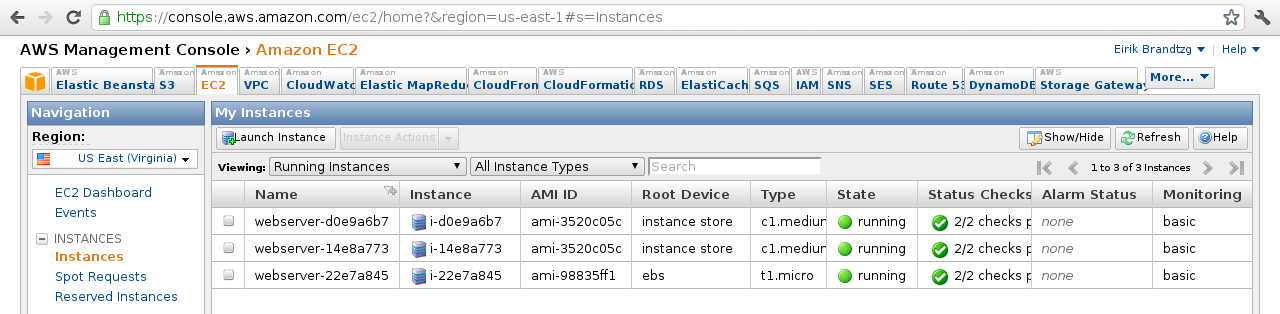
\includegraphics[width=\linewidth]{imgs/aws-console.png}
  \caption{Screenshot of \myac{AWS} console after validation provisioning.}
  \label{fig:validation-aws}
\end{figure}

\begin{figure}[tb]
  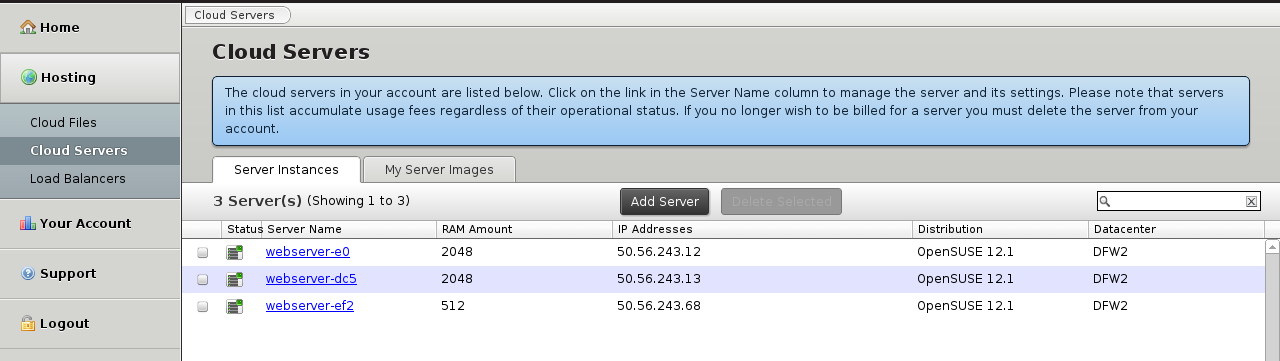
\includegraphics[width=\linewidth]{imgs/rackspace-console.png}
  \caption{Screenshot of Rackspace console after provisioning.}
  \label{fig:validation-rackspace}
\end{figure}


\paragraph{Load balancer.}
\begin{figure}[tb]
  \begin{center}
    \begin{minted}[mathescape,
                   linenos,
                   numbersep=5pt,
                   gobble=2,
                   frame=lines,
                   framesep=2mm]{json}
{
  "name": "test",
  "loadBalancer": {
    "name": "test",
    "protocol": "http",
    "loadBalancerPort": 80,
    "instancePort": 80
  }, 
  "nodes": []
}
    \end{minted}
  \end{center}
  \caption{Template including load balancer.}
  \label{list:validation-loadbalancer}
\end{figure}




\section{Comparisons}
\begin{table}
    %\begin{tabular}{ | p{2cm} | p{2cm} | p{2.5cm} | p{2cm} | p{2cm} | p{2cm} |}
  \begin{tabular*}{\textwidth}{@{\extracolsep{\fill}}| l | l | l | l | l | l |}
    %\begin{tabular*}{\textwidth}{ | l | l | l | l | l | l |}
      \hline
        \textbf{State of the art} & 
        \textbf{\citereq{software-reuse}} & 
        \textbf{\citereq{foundation}} & 
        \textbf{\citereq{mda}} & 
        \textbf{\citereq{m@rt}} & 
        \textbf{\citereq{lexical-template}} \\
      \hline
     Amazon CloudFormation & No & Hard & No & No & No \\ \hline
     CA Applogic & Yes & Easy & Yes & N & No  \\ \hline
     Libcloud & No & Hard & No & Yes & No \\ \hline
     jclouds & No & Hard & No & Yes & No \\ \hline
     OPA & Yes & Hard & No & No & No \\ \hline
     Whirr & No & Hard & No & Yes & No \\ \hline
     Deltacloud & No & Hard & No & Yes& No  \\ \hline
     CloudML & Yes & Easy & Yes & Yes & No \\ \hline
  \end{tabular*}
  \caption{Analysis}
  \label{table:analysis}
\end{table}



Comparing challenges with some selected providers and technologies from \citechap{state-of-the-art}.


\part{Conclusion}

\section{Conclusions (20)}

\note{
  Short and sharp
}

\todo{
  \begin{itemize}
    \item Summary of CloudML
    \begin{itemize}
      \item What subsection in solution solves what subsection in problem
    \end{itemize}
    \item CloudML
    \item Implementation
    \item Perspectives (2 paragraphs, can be section)
      \begin{itemize}
        \item Look into the future
          \begin{itemize}
            \item Deployments
          \end{itemize}
        \item short term
        \item long term
      \end{itemize}
  \end{itemize}
}

\begin{table}
  \begin{center}
    \caption{Result of how requirements were tackled.}
    \begin{tabular}{| l | p{12cm} |}
      \hline
        \textbf{Requirement} &
        \textbf{CloudML solution} \\
      \hline
        \citereq{software-reuse} & The engine in CloudML include and rely heavily 
                                   on an external library.
                                   This library is used to interface cloud providers
                                   with the engine.
                                   In the end this solution prevents CloudML from
                                   \emph{``reinventing the wheel''}, and keep focus 
                                   on the task at hand.
                                   \\ \hline
        \citereq{foundation} & The implementation of CloudML is developed in Scala.
                               This language introduces \emph{``state-of-the-art''}
                               features, while at the same time leverage support for
                               software industry through the \myac{JVM}.\\ \hline
        \citereq{mda} & In CloudML a model-based meta-model is designed.
                        The solution also let end users design templates with models. \\ \hline
        \citereq{lexical-template} & The engine is capable of parsing and interpreting templates.
                                     Then it configure and provision instances based on these templates.
                                     These templates are lexical, in the form of \myac{JSON}.  \\ \hline
        \citereq{m@rt} & Because of long time intervals for node provisioning CloudML introduces
                         \myac{M@RT}. This is done through asynchronous behavior of actor model,
                                      which is built into the underlying technology, Scala.
                                      Then the actor model is combined with observer pattern,
                                      enhancing the engines ability to do asynchronous callbacks. \\ \hline
        \citereq{multi-cloud} & The library \emph{jclouds} is included in the engine,
                                giving it support for $24$ providers. \\ \hline
    \end{tabular}
  \end{center}
  \label{table:results}
\end{table}



\backmatter{}
% \bibliography{mybib}
\bibliographystyle{plain}
\end{document}
